\documentclass[USenglish]{article}

\usepackage[utf8]{inputenc}%(only for the pdftex engine)
%\RequirePackage[no-math]{fontspec}[2017/03/31]%(only for the luatex or the xetex engine)
\usepackage[small]{dgruyter}
\usepackage{microtype}
\usepackage{amsmath,amssymb}
\usepackage{subcaption}
\usepackage{bbm}
%%  This file will be included when we compile the final book. You can
%%  make use of the commonly used packages and commonly defined macros
%%  from here.
%%
%%  PLEASE DO NOT CHANGE THIS FILE.
%%  PLEASE DO NOT REDFINE ANY OF THE MACROS.
%%
%%  For convenience you may wish to define your own macros in your main
%%  tex file while preparing the manuscript. However, before submitting
%%  your final file for the accepted manuscript, we will ask you to replace
%%  your macros with the full commands.
%%

\renewcommand{\email}[1]{\emailname: #1} % change the email address font style

\usepackage{mathptmx}       % selects Times Roman as basic font
\usepackage{helvet}         % selects Helvetica as sans-serif font
\usepackage{courier}        % selects Courier as typewriter font
%\usepackage{type1cm}        % activate if the above 3 fonts are
%                            % not available on your system

\usepackage{makeidx}         % allows index generation
\usepackage{graphicx}        % standard LaTeX graphics tool
                             % when including figure files
%\usepackage{multicol}        % used for the two-column index
\usepackage[bottom]{footmisc}% places footnotes at page bottom

\usepackage{latexsym}
\usepackage{amsmath}
\usepackage{amsfonts}
\usepackage{amssymb}
\usepackage{bm}

\usepackage{url}
\usepackage{algorithm}
\usepackage{algorithmic}
\usepackage[misc,geometry]{ifsym}

% Springer provides the following environments:
%   case, conjecture, corollary, definition, example, exercise, lemma,
%   note, problem, property, proposition, question, remark, solution, theorem
%   claim, proof
\renewenvironment{proof}{\noindent{\itshape Proof.}}{\smartqed\qed}

% We add two more environments:   assumption, algo
\spdefaulttheorem{assumption}{Assumption}{\upshape \bfseries}{\itshape}
\spdefaulttheorem{algo}{Algorithm}{\upshape \bfseries}{\itshape}
% Note there is also the 'algorithm' environment from the algorithm package
% which is a floating environment



% Springer defines the following commands in math mode:
%   \D upright d for differential d
%   \I upright i for imaginary unit
%   \E upright e for exponential function
%   \tens depicts tensors as sans serif upright
%   \vec depicts vectors as boldface characters instead of the arrow accent


% We add the following commonly used macros:

% vectors as boldsymbols:
\newcommand{\bsa}{{\boldsymbol{a}}}
\newcommand{\bsb}{{\boldsymbol{b}}}
\newcommand{\bsc}{{\boldsymbol{c}}}
\newcommand{\bsd}{{\boldsymbol{d}}}
\newcommand{\bse}{{\boldsymbol{e}}}
\newcommand{\bsf}{{\boldsymbol{f}}}
\newcommand{\bsg}{{\boldsymbol{g}}}
\newcommand{\bsh}{{\boldsymbol{h}}}
\newcommand{\bsi}{{\boldsymbol{i}}}
\newcommand{\bsj}{{\boldsymbol{j}}}
\newcommand{\bsk}{{\boldsymbol{k}}}
\newcommand{\bsl}{{\boldsymbol{l}}}
\newcommand{\bsm}{{\boldsymbol{m}}}
\newcommand{\bsn}{{\boldsymbol{n}}}
\newcommand{\bso}{{\boldsymbol{o}}}
\newcommand{\bsp}{{\boldsymbol{p}}}
\newcommand{\bsq}{{\boldsymbol{q}}}
\newcommand{\bsr}{{\boldsymbol{r}}}
\newcommand{\bss}{{\boldsymbol{s}}}
\newcommand{\bst}{{\boldsymbol{t}}}
\newcommand{\bsu}{{\boldsymbol{u}}}
\newcommand{\bsv}{{\boldsymbol{v}}}
\newcommand{\bsw}{{\boldsymbol{w}}}
\newcommand{\bsx}{{\boldsymbol{x}}}
\newcommand{\bsy}{{\boldsymbol{y}}}
\newcommand{\bsz}{{\boldsymbol{z}}}
\newcommand{\bsA}{{\boldsymbol{A}}}
\newcommand{\bsB}{{\boldsymbol{B}}}
\newcommand{\bsC}{{\boldsymbol{C}}}
\newcommand{\bsD}{{\boldsymbol{D}}}
\newcommand{\bsE}{{\boldsymbol{E}}}
\newcommand{\bsF}{{\boldsymbol{F}}}
\newcommand{\bsG}{{\boldsymbol{G}}}
\newcommand{\bsH}{{\boldsymbol{H}}}
\newcommand{\bsI}{{\boldsymbol{I}}}
\newcommand{\bsJ}{{\boldsymbol{J}}}
\newcommand{\bsK}{{\boldsymbol{K}}}
\newcommand{\bsL}{{\boldsymbol{L}}}
\newcommand{\bsM}{{\boldsymbol{M}}}
\newcommand{\bsN}{{\boldsymbol{N}}}
\newcommand{\bsO}{{\boldsymbol{O}}}
\newcommand{\bsP}{{\boldsymbol{P}}}
\newcommand{\bsQ}{{\boldsymbol{Q}}}
\newcommand{\bsR}{{\boldsymbol{R}}}
\newcommand{\bsS}{{\boldsymbol{S}}}
\newcommand{\bsT}{{\boldsymbol{T}}}
\newcommand{\bsU}{{\boldsymbol{U}}}
\newcommand{\bsV}{{\boldsymbol{V}}}
\newcommand{\bsW}{{\boldsymbol{W}}}
\newcommand{\bsX}{{\boldsymbol{X}}}
\newcommand{\bsY}{{\boldsymbol{Y}}}
\newcommand{\bsZ}{{\boldsymbol{Z}}}
% other commonly used boldsymbols:
\newcommand{\bsell}{{\boldsymbol{\ell}}}
\newcommand{\bszero}{{\boldsymbol{0}}} % vector of zeros
\newcommand{\bsone}{{\boldsymbol{1}}}  % vector of ones
% boldsymbol greeks:
\newcommand{\bsalpha}{{\boldsymbol{\alpha}}}
\newcommand{\bsbeta}{{\boldsymbol{\beta}}}
\newcommand{\bsgamma}{{\boldsymbol{\gamma}}}
\newcommand{\bsdelta}{{\boldsymbol{\delta}}}
\newcommand{\bsepsilon}{{\boldsymbol{\epsilon}}}
\newcommand{\bsvarepsilon}{{\boldsymbol{\varepsilon}}}
\newcommand{\bszeta}{{\boldsymbol{\zeta}}}
\newcommand{\bseta}{{\boldsymbol{\eta}}}
\newcommand{\bstheta}{{\boldsymbol{\theta}}}
\newcommand{\bsvartheta}{{\boldsymbol{\vartheta}}}
\newcommand{\bskappa}{{\boldsymbol{\kappa}}}
\newcommand{\bslambda}{{\boldsymbol{\lambda}}}
\newcommand{\bsmu}{{\boldsymbol{\mu}}}
\newcommand{\bsnu}{{\boldsymbol{\nu}}}
\newcommand{\bsxi}{{\boldsymbol{\xi}}}
\newcommand{\bspi}{{\boldsymbol{\pi}}}
\newcommand{\bsvarpi}{{\boldsymbol{\varpi}}}
\newcommand{\bsrho}{{\boldsymbol{\rho}}}
\newcommand{\bsvarrho}{{\boldsymbol{\varrho}}}
\newcommand{\bssigma}{{\boldsymbol{\sigma}}}
\newcommand{\bsvarsigma}{{\boldsymbol{\varsigma}}}
\newcommand{\bstau}{{\boldsymbol{\tau}}}
\newcommand{\bsupsilon}{{\boldsymbol{\upsilon}}}
\newcommand{\bsphi}{{\boldsymbol{\phi}}}
\newcommand{\bsvarphi}{{\boldsymbol{\varphi}}}
\newcommand{\bschi}{{\boldsymbol{\chi}}}
\newcommand{\bspsi}{{\boldsymbol{\psi}}}
\newcommand{\bsomega}{{\boldsymbol{\omega}}}
\newcommand{\bsGamma}{{\boldsymbol{\Gamma}}}
\newcommand{\bsDelta}{{\boldsymbol{\Delta}}}
\newcommand{\bsTheta}{{\boldsymbol{\Theta}}}
\newcommand{\bsLambda}{{\boldsymbol{\Lambda}}}
\newcommand{\bsXi}{{\boldsymbol{\Xi}}}
\newcommand{\bsPi}{{\boldsymbol{\Pi}}}
\newcommand{\bsSigma}{{\boldsymbol{\Sigma}}}
\newcommand{\bsUpsilon}{{\boldsymbol{\Upsilon}}}
\newcommand{\bsPhi}{{\boldsymbol{\Phi}}}
\newcommand{\bsPsi}{{\boldsymbol{\Psi}}}
\newcommand{\bsOmega}{{\boldsymbol{\Omega}}}

% Roman fonts:
\newcommand{\rma}{{\mathrm{a}}}
\newcommand{\rmb}{{\mathrm{b}}}
\newcommand{\rmc}{{\mathrm{c}}}
\newcommand{\rmd}{{\mathrm{d}}}
\newcommand{\rme}{{\mathrm{e}}}
\newcommand{\rmf}{{\mathrm{f}}}
\newcommand{\rmg}{{\mathrm{g}}}
\newcommand{\rmh}{{\mathrm{h}}}
\newcommand{\rmi}{{\mathrm{i}}}
\newcommand{\rmj}{{\mathrm{j}}}
\newcommand{\rmk}{{\mathrm{k}}}
\newcommand{\rml}{{\mathrm{l}}}
\newcommand{\rmm}{{\mathrm{m}}}
\newcommand{\rmn}{{\mathrm{n}}}
\newcommand{\rmo}{{\mathrm{o}}}
\newcommand{\rmp}{{\mathrm{p}}}
\newcommand{\rmq}{{\mathrm{q}}}
\newcommand{\rmr}{{\mathrm{r}}}
\newcommand{\rms}{{\mathrm{s}}}
\newcommand{\rmt}{{\mathrm{t}}}
\newcommand{\rmu}{{\mathrm{u}}}
\newcommand{\rmv}{{\mathrm{v}}}
\newcommand{\rmw}{{\mathrm{w}}}
\newcommand{\rmx}{{\mathrm{x}}}
\newcommand{\rmy}{{\mathrm{y}}}
\newcommand{\rmz}{{\mathrm{z}}}
\newcommand{\rmA}{{\mathrm{A}}}
\newcommand{\rmB}{{\mathrm{B}}}
\newcommand{\rmC}{{\mathrm{C}}}
\newcommand{\rmD}{{\mathrm{D}}}
\newcommand{\rmE}{{\mathrm{E}}}
\newcommand{\rmF}{{\mathrm{F}}}
\newcommand{\rmG}{{\mathrm{G}}}
\newcommand{\rmH}{{\mathrm{H}}}
\newcommand{\rmI}{{\mathrm{I}}}
\newcommand{\rmJ}{{\mathrm{J}}}
\newcommand{\rmK}{{\mathrm{K}}}
\newcommand{\rmL}{{\mathrm{L}}}
\newcommand{\rmM}{{\mathrm{M}}}
\newcommand{\rmN}{{\mathrm{N}}}
\newcommand{\rmO}{{\mathrm{O}}}
\newcommand{\rmP}{{\mathrm{P}}}
\newcommand{\rmQ}{{\mathrm{Q}}}
\newcommand{\rmR}{{\mathrm{R}}}
\newcommand{\rmS}{{\mathrm{S}}}
\newcommand{\rmT}{{\mathrm{T}}}
\newcommand{\rmU}{{\mathrm{U}}}
\newcommand{\rmV}{{\mathrm{V}}}
\newcommand{\rmW}{{\mathrm{W}}}
\newcommand{\rmX}{{\mathrm{X}}}
\newcommand{\rmY}{{\mathrm{Y}}}
\newcommand{\rmZ}{{\mathrm{Z}}}
% also commonly defined
\newcommand{\rd}{{\mathrm{d}}}
\newcommand{\ri}{{\mathrm{i}}}

% blackboards:
\newcommand{\bbA}{{\mathbb{A}}}
\newcommand{\bbB}{{\mathbb{B}}}
\newcommand{\bbC}{{\mathbb{C}}}
\newcommand{\bbD}{{\mathbb{D}}}
\newcommand{\bbE}{{\mathbb{E}}}
\newcommand{\bbF}{{\mathbb{F}}}
\newcommand{\bbG}{{\mathbb{G}}}
\newcommand{\bbH}{{\mathbb{H}}}
\newcommand{\bbI}{{\mathbb{I}}}
\newcommand{\bbJ}{{\mathbb{J}}}
\newcommand{\bbK}{{\mathbb{K}}}
\newcommand{\bbL}{{\mathbb{L}}}
\newcommand{\bbM}{{\mathbb{M}}}
\newcommand{\bbN}{{\mathbb{N}}}
\newcommand{\bbO}{{\mathbb{O}}}
\newcommand{\bbP}{{\mathbb{P}}}
\newcommand{\bbQ}{{\mathbb{Q}}}
\newcommand{\bbR}{{\mathbb{R}}}
\newcommand{\bbS}{{\mathbb{S}}}
\newcommand{\bbT}{{\mathbb{T}}}
\newcommand{\bbU}{{\mathbb{U}}}
\newcommand{\bbV}{{\mathbb{V}}}
\newcommand{\bbW}{{\mathbb{W}}}
\newcommand{\bbX}{{\mathbb{X}}}
\newcommand{\bbY}{{\mathbb{Y}}}
\newcommand{\bbZ}{{\mathbb{Z}}}
% commonly used shortcuts:
\newcommand{\C}{{\mathbb{C}}} % complex numbers
\newcommand{\F}{{\mathbb{F}}} % field, finite field
\newcommand{\N}{{\mathbb{N}}} % natural numbers {1, 2, ...}
\newcommand{\Q}{{\mathbb{Q}}} % rationals
\newcommand{\R}{{\mathbb{R}}} % reals
\newcommand{\Z}{{\mathbb{Z}}} % integers
% more commonly used shortcuts:
\newcommand{\CC}{{\mathbb{C}}} % complex numbers
\newcommand{\FF}{{\mathbb{F}}} % field, finite field
\newcommand{\NN}{{\mathbb{N}}} % natural numbers {1, 2, ...}
\newcommand{\QQ}{{\mathbb{Q}}} % rationals
\newcommand{\RR}{{\mathbb{R}}} % reals
\newcommand{\ZZ}{{\mathbb{Z}}} % integers
% more commonly used shortcuts:
\newcommand{\EE}{{\mathbb{E}}}
\newcommand{\PP}{{\mathbb{P}}}
\newcommand{\TT}{{\mathbb{T}}}
\newcommand{\VV}{{\mathbb{V}}}
% and even more commonly used shortcuts:
\newcommand{\Complex}{{\mathbb{C}}}
\newcommand{\Integer}{{\mathbb{Z}}}
\newcommand{\Natural}{{\mathbb{N}}}
\newcommand{\Rational}{{\mathbb{Q}}}
\newcommand{\Real}{{\mathbb{R}}}
% indicator boldface 1:
\DeclareSymbolFont{bbold}{U}{bbold}{m}{n}
\DeclareSymbolFontAlphabet{\mathbbold}{bbold}
\newcommand{\ind}{{\mathbbold{1}}}
\newcommand{\bbone}{{\mathbbold{1}}}


% calligraphic letters:
\newcommand{\cala}{{\mathcal{a}}}
\newcommand{\calb}{{\mathcal{b}}}
\newcommand{\calc}{{\mathcal{c}}}
\newcommand{\cald}{{\mathcal{d}}}
\newcommand{\cale}{{\mathcal{e}}}
\newcommand{\calf}{{\mathcal{f}}}
\newcommand{\calg}{{\mathcal{g}}}
\newcommand{\calh}{{\mathcal{h}}}
\newcommand{\cali}{{\mathcal{i}}}
\newcommand{\calj}{{\mathcal{j}}}
\newcommand{\calk}{{\mathcal{k}}}
\newcommand{\call}{{\mathcal{l}}}
\newcommand{\calm}{{\mathcal{m}}}
\newcommand{\caln}{{\mathcal{n}}}
\newcommand{\calo}{{\mathcal{o}}}
\newcommand{\calp}{{\mathcal{p}}}
\newcommand{\calq}{{\mathcal{q}}}
\newcommand{\calr}{{\mathcal{r}}}
\newcommand{\cals}{{\mathcal{s}}}
\newcommand{\calt}{{\mathcal{t}}}
\newcommand{\calu}{{\mathcal{u}}}
\newcommand{\calv}{{\mathcal{v}}}
\newcommand{\calw}{{\mathcal{w}}}
\newcommand{\calx}{{\mathcal{x}}}
\newcommand{\caly}{{\mathcal{y}}}
\newcommand{\calz}{{\mathcal{z}}}
\newcommand{\calA}{{\mathcal{A}}}
\newcommand{\calB}{{\mathcal{B}}}
\newcommand{\calC}{{\mathcal{C}}}
\newcommand{\calD}{{\mathcal{D}}}
\newcommand{\calE}{{\mathcal{E}}}
\newcommand{\calF}{{\mathcal{F}}}
\newcommand{\calG}{{\mathcal{G}}}
\newcommand{\calH}{{\mathcal{H}}}
\newcommand{\calI}{{\mathcal{I}}}
\newcommand{\calJ}{{\mathcal{J}}}
\newcommand{\calK}{{\mathcal{K}}}
\newcommand{\calL}{{\mathcal{L}}}
\newcommand{\calM}{{\mathcal{M}}}
\newcommand{\calN}{{\mathcal{N}}}
\newcommand{\calO}{{\mathcal{O}}}
\newcommand{\calP}{{\mathcal{P}}}
\newcommand{\calQ}{{\mathcal{Q}}}
\newcommand{\calR}{{\mathcal{R}}}
\newcommand{\calS}{{\mathcal{S}}}
\newcommand{\calT}{{\mathcal{T}}}
\newcommand{\calU}{{\mathcal{U}}}
\newcommand{\calV}{{\mathcal{V}}}
\newcommand{\calW}{{\mathcal{W}}}
\newcommand{\calX}{{\mathcal{X}}}
\newcommand{\calY}{{\mathcal{Y}}}
\newcommand{\calZ}{{\mathcal{Z}}}

% Euler fraks:
\newcommand{\fraka}{{\mathfrak{a}}}
\newcommand{\frakb}{{\mathfrak{b}}}
\newcommand{\frakc}{{\mathfrak{c}}}
\newcommand{\frakd}{{\mathfrak{d}}}
\newcommand{\frake}{{\mathfrak{e}}}
\newcommand{\frakf}{{\mathfrak{f}}}
\newcommand{\frakg}{{\mathfrak{g}}}
\newcommand{\frakh}{{\mathfrak{h}}}
\newcommand{\fraki}{{\mathfrak{i}}}
\newcommand{\frakj}{{\mathfrak{j}}}
\newcommand{\frakk}{{\mathfrak{k}}}
\newcommand{\frakl}{{\mathfrak{l}}}
\newcommand{\frakm}{{\mathfrak{m}}}
\newcommand{\frakn}{{\mathfrak{n}}}
\newcommand{\frako}{{\mathfrak{o}}}
\newcommand{\frakp}{{\mathfrak{p}}}
\newcommand{\frakq}{{\mathfrak{q}}}
\newcommand{\frakr}{{\mathfrak{r}}}
\newcommand{\fraks}{{\mathfrak{s}}}
\newcommand{\frakt}{{\mathfrak{t}}}
\newcommand{\fraku}{{\mathfrak{u}}}
\newcommand{\frakv}{{\mathfrak{v}}}
\newcommand{\frakw}{{\mathfrak{w}}}
\newcommand{\frakx}{{\mathfrak{x}}}
\newcommand{\fraky}{{\mathfrak{y}}}
\newcommand{\frakz}{{\mathfrak{z}}}
\newcommand{\frakA}{{\mathfrak{A}}}
\newcommand{\frakB}{{\mathfrak{B}}}
\newcommand{\frakC}{{\mathfrak{C}}}
\newcommand{\frakD}{{\mathfrak{D}}}
\newcommand{\frakE}{{\mathfrak{E}}}
\newcommand{\frakF}{{\mathfrak{F}}}
\newcommand{\frakG}{{\mathfrak{G}}}
\newcommand{\frakH}{{\mathfrak{H}}}
\newcommand{\frakI}{{\mathfrak{I}}}
\newcommand{\frakJ}{{\mathfrak{J}}}
\newcommand{\frakK}{{\mathfrak{K}}}
\newcommand{\frakL}{{\mathfrak{L}}}
\newcommand{\frakM}{{\mathfrak{M}}}
\newcommand{\frakN}{{\mathfrak{N}}}
\newcommand{\frakO}{{\mathfrak{O}}}
\newcommand{\frakP}{{\mathfrak{P}}}
\newcommand{\frakQ}{{\mathfrak{Q}}}
\newcommand{\frakR}{{\mathfrak{R}}}
\newcommand{\frakS}{{\mathfrak{S}}}
\newcommand{\frakT}{{\mathfrak{T}}}
\newcommand{\frakU}{{\mathfrak{U}}}
\newcommand{\frakV}{{\mathfrak{V}}}
\newcommand{\frakW}{{\mathfrak{W}}}
\newcommand{\frakX}{{\mathfrak{X}}}
\newcommand{\frakY}{{\mathfrak{Y}}}
\newcommand{\frakZ}{{\mathfrak{Z}}}
% sets as Euler fraks:
\newcommand{\seta}{{\mathfrak{a}}}
\newcommand{\setb}{{\mathfrak{b}}}
\newcommand{\setc}{{\mathfrak{c}}}
\newcommand{\setd}{{\mathfrak{d}}}
\newcommand{\sete}{{\mathfrak{e}}}
\newcommand{\setf}{{\mathfrak{f}}}
\newcommand{\setg}{{\mathfrak{g}}}
\newcommand{\seth}{{\mathfrak{h}}}
\newcommand{\seti}{{\mathfrak{i}}}
\newcommand{\setj}{{\mathfrak{j}}}
\newcommand{\setk}{{\mathfrak{k}}}
\newcommand{\setl}{{\mathfrak{l}}}
\newcommand{\setm}{{\mathfrak{m}}}
\newcommand{\setn}{{\mathfrak{n}}}
\newcommand{\seto}{{\mathfrak{o}}}
\newcommand{\setp}{{\mathfrak{p}}}
\newcommand{\setq}{{\mathfrak{q}}}
\newcommand{\setr}{{\mathfrak{r}}}
\newcommand{\sets}{{\mathfrak{s}}}
\newcommand{\sett}{{\mathfrak{t}}}
\newcommand{\setu}{{\mathfrak{u}}}
\newcommand{\setv}{{\mathfrak{v}}}
\newcommand{\setw}{{\mathfrak{w}}}
\newcommand{\setx}{{\mathfrak{x}}}
\newcommand{\sety}{{\mathfrak{y}}}
\newcommand{\setz}{{\mathfrak{z}}}
\newcommand{\setA}{{\mathfrak{A}}}
\newcommand{\setB}{{\mathfrak{B}}}
\newcommand{\setC}{{\mathfrak{C}}}
\newcommand{\setD}{{\mathfrak{D}}}
\newcommand{\setE}{{\mathfrak{E}}}
\newcommand{\setF}{{\mathfrak{F}}}
\newcommand{\setG}{{\mathfrak{G}}}
\newcommand{\setH}{{\mathfrak{H}}}
\newcommand{\setI}{{\mathfrak{I}}}
\newcommand{\setJ}{{\mathfrak{J}}}
\newcommand{\setK}{{\mathfrak{K}}}
\newcommand{\setL}{{\mathfrak{L}}}
\newcommand{\setM}{{\mathfrak{M}}}
\newcommand{\setN}{{\mathfrak{N}}}
\newcommand{\setO}{{\mathfrak{O}}}
\newcommand{\setP}{{\mathfrak{P}}}
\newcommand{\setQ}{{\mathfrak{Q}}}
\newcommand{\setR}{{\mathfrak{R}}}
\newcommand{\setS}{{\mathfrak{S}}}
\newcommand{\setT}{{\mathfrak{T}}}
\newcommand{\setU}{{\mathfrak{U}}}
\newcommand{\setV}{{\mathfrak{V}}}
\newcommand{\setW}{{\mathfrak{W}}}
\newcommand{\setX}{{\mathfrak{X}}}
\newcommand{\setY}{{\mathfrak{Y}}}
\newcommand{\setZ}{{\mathfrak{Z}}}

% other commonly defined commands:
\newcommand{\wal}{{\rm wal}}
\newcommand{\floor}[1]{\left\lfloor #1 \right\rfloor} % floor
\newcommand{\ceil}[1]{\left\lceil #1 \right\rceil}    % ceil
\DeclareMathOperator{\cov}{Cov}
\DeclareMathOperator{\var}{Var}
\providecommand{\argmin}{\operatorname*{argmin}}
\providecommand{\argmax}{\operatorname*{argmax}}


\usepackage[notref,notcite]{showkeys}

%% Beginning of author included packages and defined macros
\usepackage{color,mathtools,bbm,xspace,natbib}
\usepackage{algpseudocode}
\usepackage{algorithm, algorithmicx}
\usepackage[usenames,dvipsnames,svgnames,table]{xcolor}
\algnewcommand\algorithmicparam{\textbf{Parameters:}}
\algnewcommand\PARAM{\item[\algorithmicparam]}
\algnewcommand\algorithmicinput{\textbf{Input:}}
\algnewcommand\INPUT{\item[\algorithmicinput]}
%\algnewcommand\STATE{\item}
\algnewcommand\RETURN{\State \textbf{Return }}

\theoremstyle{dgthm}
\newtheorem{theorem}{Theorem}
\theoremstyle{dgthm}
\newtheorem{lemma}{Lemma}
\theoremstyle{dgthm}
\newtheorem{corollary}{Corollary}
\theoremstyle{dgthm}
\newtheorem{proposition}{Proposition}
\theoremstyle{dgdef}
\newtheorem{remark}{Remark}
\theoremstyle{definition}
\newtheorem{exmp}{Example}

\DeclareMathOperator{\SOL}{SOL}
\DeclareMathOperator{\APP}{APP}
\DeclareMathOperator{\ALG}{ALG}
\DeclareMathOperator{\ERR}{ERR}
\newcommand{\dataN}{\bigl(\hf(\bsk_i)\bigr)_{i=1}^n}
\newcommand{\dataNj}{\bigl(\hf(\bsk_i)\bigr)_{i=1}^{n_j}}
\newcommand{\dataNjd}{\bigl(\hf(\bsk_i)\bigr)_{i=1}^{n_{j^\dagger}}}
\newcommand{\ERRN}{\ERR\bigl(\dataN,n\bigr)}
\newcommand{\ERRNj}{\ERR\bigl(\dataNj,n_j\bigr)}
\newcommand{\ERRNjd}{\ERR\bigl(\dataNjd,n_{j^\dagger}\bigr)}
\DeclareMathOperator{\COST}{COST}
\DeclareMathOperator{\COMP}{COMP}
\newcommand{\hf}{\widehat{f}}
\newcommand{\hg}{\widehat{g}}
\newcommand{\tu}{\Tilde{u}}
\newcommand{\tv}{\Tilde{v}}
\newcommand{\tcalJ}{\widetilde{\calJ}}
\newcommand{\tcalK}{\widetilde{\calK}}
\newcommand{\tlambda}{\Tilde{\lambda}}
\newcommand{\tbbK}{\widetilde{\bbK}}
\newcommand{\lo}{\textup{lo}}
\newcommand{\up}{\textup{up}}
\newcommand{\E}{\textup{e}}
\def\abs#1{\ensuremath{\left \lvert #1 \right \rvert}}
\newcommand{\normabs}[1]{\ensuremath{\lvert #1 \rvert}}
\newcommand{\bigabs}[1]{\ensuremath{\bigl \lvert #1 \bigr \rvert}}
\newcommand{\Bigabs}[1]{\ensuremath{\Bigl \lvert #1 \Bigr \rvert}}
\newcommand{\biggabs}[1]{\ensuremath{\biggl \lvert #1 \biggr \rvert}}
\newcommand{\Biggabs}[1]{\ensuremath{\Biggl \lvert #1 \Biggr \rvert}}
\newcommand{\norm}[2][{}]{\ensuremath{\left \lVert #2 \right \rVert}_{#1}}
\newcommand{\normnorm}[2][{}]{\ensuremath{\lVert #2 \rVert}_{#1}}
\newcommand{\bignorm}[2][{}]{\ensuremath{\bigl \lVert #2 \bigr \rVert}_{#1}}
\newcommand{\Bignorm}[2][{}]{\ensuremath{\Bigl \lVert #2 \Bigr \rVert}_{#1}}
\newcommand{\biggnorm}[2][{}]{\ensuremath{\biggl \lVert #2 \biggr \rVert}_{#1}}
\newcommand{\ip}[3][{}]{\ensuremath{\left \langle #2, #3 \right \rangle_{#1}}}
\newcommand{\FredNote}[1]{{\color{blue}Fred: #1}}
\newcommand{\YuhanNote}[1]{{\color{magenta}Yuhan: #1}}
\newcommand{\PeterNote}[1]{{\color{orange}Peter: #1}}
\newcommand{\SimonNote}[1]{{\color{purple}Simon: #1}}
\newcommand{\tLambda}{\widetilde{\Lambda}}
%\newcommand{\HickernellFJ}{Hickernell}

\allowdisplaybreaks

%% End of author included packages and defined macros

\begin{document}

  %\articletype{...}

  \author[1]{Yuhan Ding}
  \author*[2]{Fred J. Hickernell}
  \author[3]{Peter Kritzer} 
  \author[4]{Simon Mak}
  \runningauthor{Y. Ding, F. J. Hickernell, P. Kritzer, and S. Mak}
  \affil[1]{Department of Mathematics, 
  Misericorida University, 301 Lake Street, Dallas, PA 18704 USA}
  \affil[2]{Department of Applied Mathematics, Illinois Institute of Technology, RE 220, 10 W.\ 32${}\text{nd}$ Street, Chicago, IL 60616 USA}
  \affil[3]{Johann Radon Institute for Computational and Applied Mathematics (RICAM), 
  Austrian Academy of Sciences, Altenbergerstr. 69, 4040 Linz, Austria}
  \affil[4]{H. Milton Stewart School of Industrial and Systems Engineering, Georgia Institute of Technology, 755 Ferst Drive, Atlanta, GA 30332 USA}
  \title{Adaptive Approximation for Multivariate Linear Problems with Inputs Lying in a Cone}
  \runningtitle{Adaptive Approximation}
  \subtitle{...}
  \abstract{...}
  %\keywords{...}
  %\classification[PACS]{...}
  %\communicated{...}
  %\dedication{...}
  %\received{...}
  %\accepted{...}
  %\journalname{...}
  %\journalyear{...}
  %\journalvolume{..}
  %\journalissue{..}
  \startpage{1}
  \aop
  %\DOI{...}

\maketitle


%%%%%%%%%%%%%%%%%%%%%%%%%%%%
\section{Introduction} 
%%%%%%%%%%%%%%%%%%%%%%%%%%%%

In many situations, adaptive algorithms can be rigorously shown to perform \emph{essentially no better} than non-adaptive algorithms.  Yet, in practice adaptive algorithms are appreciated because they relieve the user from stipulating the computational effort required to achieve the desired accuracy.  The key to resolving this seeming contradiction is to construct a theory based on assumptions that favor adaptive algorithms. We do that here.

Adaptive algorithms infer the necessary computational effort based on the function data sampled.  Adaptive algorithms may perform better than non-adaptive algorithms if the set of input functions is not convex. We construct adaptive algorithms for general multivariate linear problems where the input functions lie in non-convex cones.  Our algorithms use series coefficients of the input function to construct an approximate solution that satisfies an absolute error tolerance.  We show our algorithms to be essentially optimal.  We derive conditions under which the problem is tractable.  In the remainder of this section we define the problem and essential notation.

%%%%%%%%%%%%%%%%%%%%%%%%%%%%%%%%%%%%%%%%%%%%%%%%%%%%%%%%%%%%%%%%%%%%%%%%%%%%%%%%%%%%
\subsection{An Illustrative Example}
%%%%%%%%%%%%%%%%%%%%%%%%%%%%%%%%%%%%%%%%%%%%%%%%%%%%%%%%%%%%%%%%%%%%%%%%%%%%%%%%%%%%

Consider the case of approximating functions defined over $[-1,1]^d$, using a Chebyshev polynomial basis.  The input function is denoted $f$, and the solution is $\SOL(f) = f$ in this case
	\begin{align*}
	f &  = \sum_{\bsk \in \bbN_0^d} \widehat{f}(\bsk) u_\bsk =: \SOL(f) \\
    u_\bsk & := \prod_{\ell =1}^d \tu_{k_\ell} , & \tu_{k}(x) & := \begin{cases} 1, & k =0 ,\\
	x, & k=1,\\
	2x \tu_{k-1}(x)-\tu_{k-2}(x), & k = 2, 3, \ldots.
	\end{cases}
	\end{align*}
If one can observe the series coefficients, then $f$ can be approximated by a finite sum.  However, one should have some notion of which terms in the infinite series for $f$ are more important.  Let 
\begin{equation*}
    \lambda_\bsk := \prod_{\ell =1}^d \frac{1}{\max(1,k^r_\ell)}, \qquad \norm[\calF]{f} := \norm[2]{\left(\frac{\hf(\bsk)}{\lambda_{\bsk}}\right)_{\bsk \in \N_0^d}}.
\end{equation*}
By this definition, an input function with modest sized norm must have series coefficients that decay quickly enough as the degree of the polynomial increases.  The assumed decay is quicker for larger $r$, and this assumed decay governs the assumed smoothness of the input functions.  

The weights, $\lambda_{\bsk}$, can be ordered,
\begin{equation} \label{DHKM:lambda_order}
    \lambda_{\bsk_1} \ge \lambda_{\bsk_2} \ge \cdots >0,
\end{equation}
which then implies an ordering of the wavenumbers.  Given this ordering, it is natural to approximate the solution using the first $n$ series coefficients as follows:
\begin{equation} \label{DHKM:Ex_APP_def}
   \APP(f,n) := \sum_{i=1}^n \hf(\bsk_i) u_{\bsk_i} \quad \forall n \in \N.
\end{equation}
The error of this approximation can be defined as 
\begin{gather*}
    \norm[\calG]{\SOL(f) - \APP(f,n)} = \norm[2]{\bigl(\hf(\bsk_i) \bigr)_{i=n+1}^{\infty}}, \\
    \text{where}\qquad
    \norm[\calG]{\sum_{\bsk \in \N_0^d} \hg(\bsk) u_{\bsk}} : = \norm[2]{\bigl(\hg(\bsk) \bigr)_{\bsk \in \N_0^d}}.
\end{gather*}

If one has a fixed data budget, $n$, then choosing approximation $\APP(f,n)$ is appropriate.  However, often one has an error tolerance, $\varepsilon$, for which one desires an algorithm, $\ALG(f,\varepsilon)$, which satisfies
\begin{equation*}
    \norm[\calG]{\SOL(f) - \ALG(f,\varepsilon)} \le \varepsilon.
\end{equation*}
Such an algorithm must have a rule of choosing the correct $n$---depending on $f$ and $\varepsilon$---so that $\ALG(f,\varepsilon) = \APP(f,n)$.  Choosing such a rule, choosing a set $\calC$ of input functions for which the rule is valid,  characterizing the information cost of $\ALG$, and determining whether $\ALG$ has optimal information cost, and understanding the dependence of this cost on the the number of input variables, $d$, as well as the error tolerance, $\varepsilon$, are all objectives of this chapter.


%%%%%%%%%%%%%%%%%%%%%%%%%%%%%%%%%%%%%%%%%%%%%%%%%%%%%%%%%%%%%%%%%%%%%%%%%%%%%%%%%%%%
\subsection{General Linear Problem}
%%%%%%%%%%%%%%%%%%%%%%%%%%%%%%%%%%%%%%%%%%%%%%%%%%%%%%%%%%%%%%%%%%%%%%%%%%%%%%%%%%%%
Our general linear problem is defined by a solution operator mapping an input function to an output, $\SOL:\calF \to \calG$.  As in the illustrative example above, the Banach spaces of inputs and outputs are defined by series expansions:
\begin{gather}
    \calF = \left \{f = \sum_{\bsk \in \mathbb{K}} \hf(\bsk) u_{\bsk} : \norm[\calF]{f} : = \norm[\rho]{\left( \frac{\hf(\bsk)}{\lambda_{\bsk}} \right)_{\bsk \in \mathbb{K}}} < \infty \right\}, \quad 1 \le \rho \le \infty, \\
    \calG = \left \{g = \sum_{\bsk \in \mathbb{K}} \hg(\bsk) v_{\bsk} : \norm[\calG]{g} : = \norm[\tau]{\bigl(  \hg(\bsk)  \bigr)_{\bsk \in \mathbb{K}}} < \infty \right\}, \quad 1 \le \tau \le \rho.
\end{gather}
Here, $\{u_{\bsk}\}_{\bsk \in \mathbb{K}}$ is a basis for the input Banach space $\calF$, and $\{v_{\bsk}\}_{\bsk \in \mathbb{K}}$ is a basis for the output Banach space $\calG$. These bases are defined to match the solution operator:
\begin{equation} \label{DHKM:basis_relate}
    \SOL(u_{\bsk}) = v_{\bsk} \qquad \forall \bsk \in \mathbb{K},
\end{equation}
where $\mathbb{K}$ is a general index set. The $\lambda_{\bsk}$ represent the importance of the series coefficients of the input function.  The larger $\lambda_{\bsk}$ is, the more important $\hf(\bsk)$ is.

Although this problem formulation is quite general in some aspects, condition \eqref{DHKM:basis_relate} is somewhat restrictive.  In theory, the choice of basis can be made via the singular value decomposition, but in practice, if the norms of $\calF$ and $\calG$ are typical, the bases satisfying \eqref{DHKM:basis_relate} may be difficult to identify explicitly.

To facilitate our derivations below, we establish the following lemma, which follows from H\"older's inequality:

\begin{lemma} \label{DHKM:Key_Lem}
Let $\calK$ be some proper or improper subset of $\bbK$. Moreover, let $\rho'$ be defined by the relation
\begin{equation*}
    \frac 1\rho + \frac 1 {\rho'} = \frac 1 \tau, \qquad \text{i.e., } \rho' = \frac{\rho \tau}{\rho - \tau},
\end{equation*}
so $\tau \le \rho' \le \infty$.  Let $\Lambda =  \bignorm[\rho']{\bigl(  \lambda_{\bsk}  \bigr)_{\bsk \in \calK}}$.  Then the following are true for $f = \sum_{\bsk \in \calK} \hf(\bsk) u_{\bsk}$:
\begin{equation}
\label{DHKM:SOL_ineq}
    \norm[\calG]{\SOL(f)} = \norm[\tau]{\bigl(\hf(\bsk) \bigr)_{\bsk \in \calK}} \le \norm[\calF]{f} \, \Lambda,
    \end{equation}
    \begin{multline}
    \label{DHKM:SOL_tight_ineq}
    \bigabs{\hf(\bsk)} = \begin{cases}
    \displaystyle 
    \frac{R \lambda_{\bsk}^{\rho'/\rho + 1}}{\Lambda^{\rho'/\rho}}, & \forall \bsk \in \calK, \quad  \rho'<\infty \\
    R \Lambda \delta_{\bsk,\bsk^*}, & \forall \bsk \in \calK, \ \bsk^* \in \calK \text{ satisfies } \lambda_{\bsk^*} = \Lambda, \quad \rho' = \infty,
    \end{cases}
   \\ 
    \implies  \ \ \norm[\calF]{f} = R \ \& \ \norm[\calG]{\SOL(f)} = R \Lambda.
    \end{multline}
    
\PeterNote{Please excuse me for asking stupid questions all the time, but I was wondering: if $\rho'=\infty$, how would the formula for the $\hf (\bsk)$ in (7) look like? We would have $\infty$ in the exponents.}
\FredNote{How does it look now?}
Equality \eqref{DHKM:SOL_tight_ineq} illustrates how inequality \eqref{DHKM:SOL_ineq} may be made tight.
\end{lemma}
\begin{proof}
We give the proof for $\rho' < \infty$.  The proof for $\rho' = \infty$ follows similiarly. 
The proof of inequality \eqref{DHKM:SOL_ineq} proceeds by applying H\"older's inequality:  
\begin{align}
    \label{DHKM:SOL_A}
    \norm[\calG]{\SOL(f)}  
    & = \biggnorm[\calG]{\sum_{\bsk \in \calK} \hf(\bsk) v_{\bsk}} = \norm[\tau]{\bigl(  \hf(\bsk)  \bigr)_{\bsk \in \calK}}  = \left [\sum_{\bsk \in \calK}  \left\lvert\frac{\hf(\bsk)}{\lambda_{\bsk}} \right\rvert^{\tau} \lambda_{\bsk}^{\tau} \right]^{1/\tau} \\
    \nonumber
    & \le \biggnorm[\rho]{\biggl(  \frac{\hf(\bsk)}{\lambda_{\bsk}}  \biggr)_{\bsk \in \calK}} \, \bignorm[\rho']{\bigl(  \lambda_{\bsk}  \bigr)_{\bsk \in \calK}} \qquad \text{since }\frac 1\rho + \frac 1 {\rho'} = \frac 1 \tau \\
    \nonumber
    & = \norm[\calF]{f} \, \Lambda.
\end{align}
Substituting the formula for $\bigabs{\hf(\bsk)}$ in \eqref{DHKM:SOL_tight_ineq} into equation \eqref{DHKM:SOL_A} and applying the relationship between $\rho$, $\rho'$, and $\tau$ yields
\begin{equation*}
       \norm[\calG]{\SOL(f)}  
    =  \frac{R \bignorm[\tau]{\bigl(  \lambda_{\bsk}^{\rho'/\rho + 1}  \bigr)_{\bsk \in \calK}}} {\Lambda^{\rho'/\rho}} 
    = \frac{R \bignorm[\rho']{\bigl(  \lambda_{\bsk}  \bigr)_{\bsk \in \calK}}^{\rho'/\rho + 1}}
    {\Lambda^{\rho'/\rho}} = R \Lambda.
\end{equation*}
Moreover,
\begin{equation*}
    \norm[\calF]{f}  
    = \norm[\rho]{\left( \frac{\hf(\bsk)}{\lambda_{\bsk}} \right)_{\bsk \in \calK}}
    = \frac{R \bignorm[\rho]{\bigl(  \lambda_{\bsk}^{\rho'/\rho}  \bigr)_{\bsk \in \calK}}}{\Lambda^{\rho'/\rho}} 
    = \frac{R \bignorm[\rho']{\bigl(  \lambda_{\bsk}  \bigr)_{\bsk \in \calK}}^{\rho'/\rho}}
    {\Lambda^{\rho'/\rho}} = R.
\end{equation*}
This completes the proof.
\end{proof} \

%\hspace{\parindent} 
Based on this lemma and taking $\calK = \bbK$, the norm of the solution operator can be expressed in terms of the $\lambda_\bsk$ as follows:
\begin{equation} \label{DHKM:SOLNorm}
    \norm[\calF \to \calG]{\SOL}  = \sup_{\norm[\calF]{f} \le 1} \norm[\calG]{\SOL(f)} = \bignorm[\rho']{\bigl(  \lambda_{\bsk}  \bigr)_{\bsk \in \mathbb{K}}}.
\end{equation}
The $\lambda_{\bsk}$ define the smoothness of the input space and are assumed to have a known order:
\begin{equation} \label{DHKM:lambda_order}
    \lambda_{\bsk_1} \ge \lambda_{\bsk_2} \ge \cdots >0.
\end{equation}
We assume that all $\lambda_{\bsk_i}$ are positive to avoid the trivial case where the problem can be solved by knowing a finite number of series coefficients.
An optimal approximation  based on $n$ series coefficients of the input function can be defined in terms of the series coefficients of the input function corresponding to the largest $\lambda_{\bsk}$ as follows:
\begin{equation} \label{DHKM:APP_def}
    \APP : \calF \times \N_0 \to \calG, \quad  \APP(f,0) = 0, \ \ \APP(f,n) := \sum_{i=1}^n \hf(\bsk_i) v_{\bsk_i} \ \forall n \in \N.
\end{equation}

\begin{theorem} \label{DHKM:APP_optimality_thm} Let $\calB_{R} : = \{ f \in \calF : \norm[\calF]{f} \le R \}$ denote the ball of radius $R$ in the space of input functions.  The error of the approximation defined in \eqref{DHKM:APP_def} is bounded tightly above as 
\begin{equation} \label{DHKM:APP_errorBd}
    \sup_{f \in \calB_R} \norm[\calG]{\SOL(f) - \APP(f,n)}  \le R \, \bignorm[\rho']{\bigl(  \lambda_{\bsk_i}  \bigr)_{i = n+1}^{\infty}}.
\end{equation}
Moreover, the worst case error over $\calB_R$ of any approximation based on $n$ series coefficients of the input function, $\APP'(\cdot,n)$, can be no smaller.
\end{theorem}

\begin{proof}
The proof of \eqref{DHKM:APP_errorBd} follows from an argument similar to that used to derive 
\eqref{DHKM:SOLNorm}.  The optimality of $\APP$ follows by bounding the error of an arbitrary approximation, $\APP'$ applied to functions that mimic the zero function.

 Let $\APP'(0,n)$ depend on the series coefficients indexed by $\calJ  = \{\bsk'_1, \ldots, \bsk'_n\}$.  Use Lemma \ref{DHKM:Key_Lem} with $\calK = \bbK \setminus \calJ$ to choose $f$ to satisfy the following conditions:
\begin{gather*}
    \hf(\bsk'_1) = \cdots = \hf(\bsk'_n) = 0, \qquad \norm[\calF]{f} = R, \\ \Bignorm[\tau]{\bigl(\hf(\bsk)\bigr)_{\bsk \notin \calJ}}
    = \norm[\rho]{\left( \frac{\hf(\bsk)}{\lambda_{\bsk}} \right)_{\bsk \notin \calJ}} \,
    \norm[\rho']{\left( \lambda_{\bsk} \right)_{\bsk \notin \calJ}}.
\end{gather*}
Then $\APP'(\pm f,n) = \APP'(0,n)$, and
\begin{align*}
\MoveEqLeft{\max_{\pm} \norm[\calG]{\SOL(\pm f) - \APP'(\pm f,n)} =  \max_{\pm} \norm[\calG]{\SOL(\pm f) - \APP'(0,n)}} \\
& \ge \frac 12 \left [ \norm[\calG]{\SOL(f) - \APP'(0,n)} 
+ \norm[\calG]{- \SOL(f) - \APP'(0,n)}\right] \\
& \ge \norm[\calG]{\SOL(f)} 
 = R  \norm[\rho']{\left( \lambda_{\bsk} \right)_{\bsk \notin \calJ}} \qquad \text{by \eqref{DHKM:SOL_tight_ineq}}.
\end{align*}
The ordering of the $\lambda_{\bsk}$ implies that $\norm[\rho']{\left( \lambda_{\bsk} \right)_{\bsk \notin \calJ}}$ for arbitrary $\calJ$ can be no smaller than the case $\calJ = \{\bsk_1, \ldots, \bsk_n\}$.  This completes the proof.
\end{proof}

\hspace{\parindent} The decay rate of the approximation error in \eqref{DHKM:APP_errorBd} depends on the decay rate of the tail norm of the $\lambda_{\bsk_i}$.  This decay may be algebraic or exponential and will determine the complexity of the problem as a function of the error tolerance.  

While approximation $\APP$ is a key piece of the puzzle, our ultimate goal is an algorithm, $\ALG : \calC \subset \calF \times [0,\infty)$, satisfying the absolute error criterion
\begin{equation} \label{DHKM:err_crit}
    \norm[\calG]{\SOL(f) - \ALG(f,\varepsilon)} \le \varepsilon \qquad \forall f \in \calC.
\end{equation}
The non-adaptive Algorithm \ref{DHKM:BallAlg} satisfies this error criterion for $\calC  = \calB_R$.  

\begin{algorithm}
\caption{Non-Adaptive $\ALG$ for a Ball of Input Functions \label{DHKM:BallAlg}}
	\begin{algorithmic}
	\PARAM the ball radius, $R$; $\APP$ satisfying \eqref{DHKM:APP_errorBd}
	\INPUT a black-box function, $f$; an absolute error tolerance, $\varepsilon>0$

    \Ensure Error criterion \eqref{DHKM:err_crit} for $\calC = \calB_{R}$

    \State Choose $n^* =  \min \left \{n \in \N_0 : \bignorm[\rho']{\bigl(  \lambda_{\bsk_i}  \bigr)_{i = n+1}^{\infty}} \le \varepsilon /R \right \}$

    \RETURN $\ALG(f,\varepsilon) = \APP(f,n^*)$
\end{algorithmic}
\end{algorithm}

After defining the information cost of an algorithm and the problem complexity in the next subsection, we demonstrate that this non-adaptive algorithm is optimal when the set of inputs is chosen to be $\calC = \calB_R$. However, typically one cannot bound the norm of the input function a priori, so Algorithm \ref{DHKM:BallAlg} is impractical. 

The key difficulty is that error bound \eqref{DHKM:APP_errorBd} depends on the norm of the input function.  In contrast, we will construct  error bounds for $\APP(f,n)$ that only depend on function values.  These will lead to \emph{adaptive} algorithms $\ALG$ satisfying error criterion \eqref{DHKM:err_crit}.  For such algorithms, the set of allowable input functions, $\calC$, will be a \emph{cone}, not a ball.

Note that algorithms satisfying \eqref{DHKM:err_crit} cannot exist for $\calC = \calF$. Any algorithm must require a finite sample size, even if it is huge.  Then, there must exist some $f \in \calF$ that looks exactly like the zero function to the algorithm but for which $\norm[\calG]{\SOL(f)}$ is arbitrarily large.  Thus, algorithms satisfying the error criterion only exist for some strict subset of $\calF$, and choosing that subset well is both an art and a science.


%%%%%%%%%%%%%%%%%%%%%%%%%%%%
\subsection{Information Cost and Problem Complexity}
%%%%%%%%%%%%%%%%%%%%%%%%%%%%

The information cost of $\ALG(f,\varepsilon)$ is denoted $\COST(\ALG,f,\varepsilon)$ and defined as the number of function data---in our case series coefficients---required by $\ALG(f,\varepsilon)$.  For adaptive algorithms this cost varies with the input function $f$.  We also define the information cost of the algorithm in general, recognizing that it will tend to depend on $\norm[\calF]{f}$
\begin{equation*}
    \COST(\ALG, \calC, \varepsilon,R) : = \max_{f \in \calC \cap \calB_{R}} \COST(\ALG,f,\varepsilon).
\end{equation*}
Note that while the cost depends on $\norm[\calF]{f}$, $\ALG(f,\varepsilon)$ has no knowledge of $f$ beyond the fact that it lies in $\calC$.  It is common for $\COST(\ALG, \calC, \varepsilon,R)$ to be bounded by a power of $\varepsilon^{-1}$.

Let $\calA(\calC)$ denote the set of all possible algorithms that may be constructed using series coefficients and that \emph{satisfy error criterion \eqref{DHKM:err_crit}}.  We define the \emph{computational complexity} of a problem as the information cost of the best algorithm:
\begin{equation*}
    \COMP(\calA(\calC), \varepsilon,R) := \min_{\ALG \in \calA(\calC)} \COST(\ALG, \calC, \varepsilon,R) .
\end{equation*}
These definitions follow the information-based complexity literature \cite{TraWer98, TraWasWoz88}.
We define an algorithm to be \emph{essentially optimal} if there exists some fixed positive $\omega$ for which
\begin{equation} \label{DHKM:EssentialOpt}
    \COST(\ALG, \calC, \varepsilon,R) \le \COMP(\calA(\calC), \omega \varepsilon,R) \qquad \forall \varepsilon,R > 0.
\end{equation}
If the complexity of the problem is $\calO(\varepsilon^{-p})$, the cost of an essentially optimal algorithm is also $\calO(\varepsilon^{-p})$. If the complexity of the problem is asymptotically $c \log(1 + \varepsilon^{-1})$, then  the cost of an essentially optimal algorithm is also asymptotically $c \log(1 + \varepsilon^{-1})$. 
We will show that our adaptive algorithms are essentially optimal.

\begin{theorem}
The non-adaptive Algorithm \ref{DHKM:BallAlg} is essentially optimal for our problem when the set of input functions is $\calC = \calB_R$, specifically
\[
\COST(\ALG, \calB_R, \varepsilon,R') \le \COMP(\calA(\calB_R), \varepsilon R'/R,R') \qquad \forall \varepsilon > 0, \ 0 < R' \le R.
\]
\end{theorem}

\begin{proof}  Fix positive $\varepsilon$, $R$ and $R' \le R$.  Let $\omega = R'/R$.  From the definition of the non-adaptive Algorithm  \ref{DHKM:BallAlg}, 
\[
\COST(\ALG, \calB_R, \varepsilon,R') = n^*(\varepsilon,R) = \min \left \{n \in \N_0 : \bignorm[\rho']{\bigl(  \lambda_{\bsk_i}  \bigr)_{i = n+1}^{\infty}} \le \varepsilon /R \right \}.
\]
Construct an input function $f \in \calB_{R'}$ as in the proof of Theorem \ref{DHKM:APP_optimality_thm} with $\calJ = \{\bsk_1, \ldots, \bsk_{n^*(\omega \varepsilon,R')} \}$. By the argument in the proof of Theorem \ref{DHKM:APP_optimality_thm}, any algorithm in $\calA(\calB_{R'})$ that can approximate $\SOL(f)$ with an error no greater than $\omega \varepsilon$ must use at least $n^*(\omega \varepsilon,R')$ series coefficients.  Thus, 
\begin{align*}
\COST(\ALG, \calB_R, \varepsilon,R') & =  n^*(\varepsilon,R) 
= n^*(\varepsilon R'/R,R') = n^*(\omega \varepsilon, R')
\\
& \le \COMP(\calA(\calB_{R'}),\omega \varepsilon, R') \le  \COMP(\calA(\calB_{R}),\omega \varepsilon, R').
\end{align*}
Thus, Algorithm \ref{DHKM:BallAlg} is essentially optimal. For $R'=R \ (\omega = 1)$, we have optimality.
\end{proof}

\hspace{\parindent} This theorem illustrates how an essentially optimal algorithm for solving a problem for a ball of input functions, $\calC = \calB_R$, can be non-adaptive.  However, as alluded to above, we claim that it is impractical to know a priori which ball your input function lies in.  On the other hand, in the situations described below where $\calC$ is a cone, we will show that $\calA(\calC)$ actually contains only adaptive algorithms via the lemma below.  The proof of this lemma follows directly from the definition of non-adaptivity.

\begin{lemma} \label{DHKM:NoNonAdpatLem}
For a given set of input functions, $\calC$, if  $\calA(\calC)$ contains any non-adaptive algorithms, then for every $\varepsilon > 0$,
\begin{equation*}
    \sup_{R > 0} \COMP(\calA(\calC),\varepsilon, R) < \infty.
\end{equation*}
\end{lemma}

Consider the example in Section 1.1, we obtain
	\begin{align*}
	\textup{COMP}(\calA(\calB_{R}),\varepsilon,R) &= \textup{COST}(ALG,\calB_{R},\varepsilon,R) 
	=\min\{ n \in \N_0 : \lambda_{\bsk_{n+1}} \le \varepsilon/R \} \\
	& = \min \left\{ n \in \N_0: \prod_{\ell =1}^d \frac{1}{\max(1,k^r_{n+1,\ell})} \le \frac{\varepsilon}{R} \right\} 
	% & \lambda_{n+1} = \frac{1}{\lceil (n+1)/2 \rceil^r}.
	\end{align*}
	\YuhanNote{I can't get an explicit bound of n}
	Here, $\calG=L^2[-1,1]$.  The larger the non-negative parameter $r$ is, the faster the $\lambda_{\bsk_i}$ tend to 0 as $ i \to 0$, the more exclusive $\calB_R$ is, and the smaller  $\textup{cost}(ALG,\calB_{R},\varepsilon,R)$ is.  For $r = 0$, $\textup{cost}(ALG,\calB_{R},\varepsilon,R) = \infty$.

%%%%%%%%%%%%%%%%%%%%%%%%%%%%
\subsection{Tractability}\label{DHKM:secTractability}
%%%%%%%%%%%%%%%%%%%%%%%%%%%%



Besides understanding the dependence of the computational complexity on $\varepsilon$, we also want to understand how this quantity depends on the dimension of the domain of the input function.  Suppose that $f: \Omega^d \to \R$, for some $\Omega \subseteq \R$, and let $\calF_d$ denote the dependence of the input space on the dimension $d$.  Let the bases and $\lambda_{\bsk}$ be of product form:
\begin{gather*}
    u_{\bsk} = \tu_{1,k_1} \cdots \tu_{d,k_d}, \qquad  v_{\bsk} = \tv_{1,k_1} \cdots \tv_{d,k_d}, \\ 
    \lambda_{\bsk} = \tlambda_{1,k_1} \cdots \tlambda_{d,k_d}, \quad \forall \bsk = (k_1, \ldots, k_d) \in \bbK = \tbbK^d.
\end{gather*}
The cone of functions for which our algorithms succeed, $\calC_d$, will also depend on the dimension.  Also, $\SOL$, $\APP$, $\COST$, and $\COMP$ depend implicitly on dimension, and this dependence is sometimes indicated explicitly by the subscript $d$.

\bigskip

We would like to study how $\COMP(\calA(\calC_d), \varepsilon,R)$ 
depends on the dimension $d$ and the error threshold $\varepsilon$. This is described by defining various notions of tractability. Roughly speaking, the different tractability notions correspond to different 
ways of how the complexity $\COMP(\calA(\calC_d), \varepsilon,R)$ depends on $d$ and $\varepsilon$. Since 
the complexity is defined in terms of the best available algorithm, tractability is a property that is inherent to the problem, not to a particular algorithm. 
We define the following notions of tractability (for further information on tractability we refer to the trilogy 
\cite{NovWoz08a}, \cite{NovWoz10a}, \cite{NovWoz12a}). 

\begin{itemize}   
\item We say that the adaptive approximation problem is strongly polynomially tractable
if and only if there are non-negative $C$ and $p$ such that   
for all \ $d\in\NN,\ \varepsilon\in (0,1)$ we have   
$$   
\COMP(\calA(\calC_d), \varepsilon,R)\le C\,\varepsilon^{-p}.
$$   
The infimum of $p$ satisfying the bound above is denoted by $p^*$   
and is called the exponent of strong polynomial tractability.    
\newline \qquad   

\item    
We say that the problem is polynomially tractable
if and only if there are non-negative $C,p$, and $q$ such that   
for all \ $d\in\NN,\ \varepsilon\in (0,1)$ we have   
$$   
\COMP(\calA(\calC_d), \varepsilon,R)\le C\,d^{\,q}\,   
\varepsilon^{-p}.   
$$   
\vskip 0.5pc     
 

   
\item   
We say that the problem is weakly tractable iff    
$$   
\lim_{d+\varepsilon^{-1}\to\infty}\   
\frac{\log\, \COMP(\calA(\calC_d), \varepsilon,R)}   
{d+\varepsilon}\,=\,0.   
$$    
\end{itemize}   

Necessary and sufficient conditions on these tractability notions will be studied 
for different types of algorithms in Sections \ref{DHKM:SecPilotTract} and \ldots . 


%%%%%%%%%%%%%%%%%%%%%%%%%%%%%%%%%%%%%%%%%%%%%%%%%%%%%%%%%%%%%%%%%%%%%%%%%%%%%
%%%%%%%%%%%%%%%%%%%%%%%%%%%%%%%%%%%%%%%%%%%%%%%%%%%%%%%%%%%%%%%%%%%%%%%%%%%%%
%%%%%%%%%%%%%%%%%%%%%%%%%%%%%%%%%%%%%%%%%%%%%%%%%%%%%%%%%%%%%%%%%%%%%%%%%%%%%
%%%%%%%%%%%%%%%%%%%%%%%%%%%%%%%%%%%%%%%%%%%%%%%%%%%%%%%%%%%%%%%%%%%%%%%%%%%%%
\section{Bounding the Norm of the Input Function Based on a Pilot Sample} 
%%%%%%%%%%%%%%%%%%%%%%%%%%%%%%%%%%%%%%%%%%%%%%%%%%%%%%%%%%%%%%%%%%%%%%%%%%%%%
%%%%%%%%%%%%%%%%%%%%%%%%%%%%%%%%%%%%%%%%%%%%%%%%%%%%%%%%%%%%%%%%%%%%%%%%%%%%%
%%%%%%%%%%%%%%%%%%%%%%%%%%%%%%%%%%%%%%%%%%%%%%%%%%%%%%%%%%%%%%%%%%%%%%%%%%%%%


%%%%%%%%%%%%%%%%%%%%%%%%%%%%
\subsection{The Cone and the Optimal Algorithm}
%%%%%%%%%%%%%%%%%%%%%%%%%%%%

The premise of an adaptive algorithm is that the finite information we observe about the input function 
tells us something about what is not observed about the input function.  Let $n_1$ denote the number of pilot samples to be observed, based on the wave numbers
\begin{equation} \label{DHKM:KOnedef}
    \calK_1 := \{\bsk_1, \ldots, \bsk_{n_1} \},
\end{equation}
where the $\bsk_i$ are given by the ordering of the $\lambda_{\bsk}$ in \eqref{DHKM:lambda_order}.  Let $a$ be some constant inflation factor greater than one.  The cone of functions whose norm can be bounded well in terms of a pilot sample 
is given by
\begin{equation} \label{DHKM:pilot_cone}
    \calC = \left \{ f \in \calF : \norm[\calF]{f} \le a \norm[\rho]{\left( \frac{\hf(\bsk)}{\lambda_{\bsk}} \right)_{\bsk \in \calK_1}} \right\}.
\end{equation}

The error of $\APP(f,n)$ given in Theorem \ref{DHKM:APP_optimality_thm} can be refined by noting that the error only depends on the series coefficients numbered $n+1$ and more.  Specifically, 
\begin{equation} \label{DHKM:Refined_APP_err}
    \norm[\calG]{\SOL(f) - \APP(f,n) } \le \norm[\rho]{\left(\frac{\hf(\bsk_i)}{\lambda_{\bsk_i}}\right)_{i=n+1}^\infty}
    \bignorm[\rho']{\bigl(  \lambda_{\bsk_i}  \bigr)_{i = n+1}^{\infty}}.
\end{equation}
Moreover, by the definitions of the $\calF$-norm and $\calC$,
\begin{align*}
     \norm[\rho]{\left(\frac{\hf(\bsk_i)}{\lambda_{\bsk_i}}\right)_{i=n+1}^\infty} & =  \left[ \norm[\calF]{f}^\rho -  \norm[\rho]{\left(\frac{\hf(\bsk_i)}{\lambda_{\bsk_i}}\right)_{i=1}^n}^\rho
    \right]^{1/\rho} \qquad \forall f \in \calF \\
    &  \le  \left[ a^\rho \norm[\rho]{\left( \frac{\hf(\bsk)}{\lambda_{\bsk}} \right)_{\bsk \in \calK_1}}^\rho -  \norm[\rho]{\left(\frac{\hf(\bsk_i)}{\lambda_{\bsk_i}}\right)_{i=1}^n}^\rho
    \right]^{1/\rho} \quad \forall f \in \calC.
\end{align*}
This inequality together with \eqref{DHKM:Refined_APP_err} implies the data-based error bound 
\begin{subequations} \label{DHKM:pilot_errbd}
\begin{equation}
\norm[\calG]{\SOL(f) - \APP(f,n)}  \le \ERRN  \qquad \forall f \in \calC,
\end{equation}
where 
\begin{multline}
\ERRN \\
    : =  
    \left[ a^\rho \norm[\rho]{\left( \frac{\hf(\bsk)}{\lambda_{\bsk}} \right)_{\bsk \in \calK_1}}^\rho -  \norm[\rho]{\left(\frac{\hf(\bsk_i)}{\lambda_{\bsk_i}}\right)_{i=1}^n}^\rho \right]^{1/\rho} 
    \, \bignorm[\rho']{\bigl(  \lambda_{\bsk_i}  \bigr)_{i = n+1}^{\infty}} , 
    \\ n > n_1.
\end{multline}
\end{subequations}
This error bound decays as $\bignorm[\rho]{\bigl( f(\bsk_i)/\lambda_{\bsk_i} \bigr)_{i=1}^n}$ increases and as the tail norm of the $\lambda_{\bsk_i}$ decreases.  For this $\calC$ defined in \eqref{DHKM:pilot_cone}, Algorithm \ref{DHKM:PilotConeAlg} is successful:

\begin{algorithm}
	\caption{$\ALG$ Based on a Pilot Sample\label{DHKM:PilotConeAlg}} 
	\begin{algorithmic}
	\PARAM an initial sample size, $n_1 \in \N$; an inflation factor, $a > 1$; $\APP$ satisfying \eqref{DHKM:APP_errorBd}
		\INPUT a black-box function, $f$; an absolute error tolerance,
		$\varepsilon>0$

\Ensure Error criterion \eqref{DHKM:err_crit} for  the cone defined in \eqref{DHKM:pilot_cone}

\State Let $n \leftarrow 0$
\Repeat

\State Let $n \leftarrow n + 1$

\State Compute $\ERRN$ as defined in \eqref{DHKM:pilot_errbd}

\Until $\ERRN \le \varepsilon$

\RETURN $\ALG(f,\varepsilon) = \APP(f,n)$

\end{algorithmic}
\end{algorithm}

\begin{theorem} \label{DHKM:PilotCostThm}
Algorithm \ref{DHKM:PilotConeAlg} yields an answer satisfying absolute error criterion \eqref{DHKM:err_crit}, i.e., $\ALG \in \calA(\calC)$ for $\calC$ defined in \eqref{DHKM:pilot_cone}.  The information cost is
\begin{multline} \label{DHKM:PilotConeAlg_cost}
    \COST(\ALG,\calC,\varepsilon,R) \\
    = \min \left \{n \ge n_1 : \bignorm[\rho']{\bigl(  \lambda_{\bsk_i}  \bigr)_{i = n+1}^{\infty}} \,
    \le \varepsilon/[(a^\rho -1)^{1/\rho}R] \right \}.
\end{multline}
The computational complexity has the lower bound
\begin{equation} \label{DHKM:PilotConeAlg_comp}
        \COMP(\calA(\calC),\varepsilon,R) \ge \min \left \{n \ge n_1 : \bignorm[\rho']{\bigl(  \lambda_{\bsk_i}  \bigr)_{i = n+1}^{\infty}} \,
    \le 2\varepsilon/[(1 - 1/a) R] \right \}.
\end{equation}
Therefore, Algorithm \ref{DHKM:PilotConeAlg} is essentially optimal.  Moreover, $\calA(\calC)$ contains only adaptive algorithms.
\end{theorem}

\begin{proof} 
The upper bound on the computational cost of this algorithm is obtained by noting that 
\begin{align*}
    \MoveEqLeft{\COST(\ALG,\calC,\varepsilon,R)} \\
    & = \max_{f \in \calC \cap \calB_{R}} \min \left \{n \ge n_1 : \ERRN \le \varepsilon \right \} \\
     & \le \max_{f \in \calC \cap \calB_{R}} \min \left \{n \ge n_1 : 
     (a^\rho -1)^{1/\rho} \norm[\rho]{\left( \frac{\hf(\bsk)}{\lambda_{\bsk}} \right)_{\bsk \in \calK}} \, 
     \bignorm[\rho']{\bigl(  \lambda_{\bsk_i}  \bigr)_{i = n+1}^{\infty}}
    \le \varepsilon \right \} \\   
     & \le \min \left \{n \ge n_1 : 
     (a^\rho -1)^{1/\rho} R \bignorm[\rho']{\bigl(  \lambda_{\bsk_i}  \bigr)_{i = n+1}^{\infty}} 
    \le \varepsilon \right \},  
\end{align*}
since $\bignorm[\rho]{\bigl( \hf(\bsk)/\lambda_{\bsk} \bigr)_{\bsk \in \calK}} \le \bignorm[\rho]{\bigl( \hf(\bsk_i)/\lambda_{\bsk_i} \bigr)_{i=1}^{n}} \le  \norm[\calF]{f} \le R$ for all $f \in \calB_R$, $n \ge n_1$.  Moreover, this inequality is tight for some $f \in \calC \cap \calB_{R}$, namely, those certain $f$ for which $\hf(\bsk_i) = 0$ for $i > n_1$.  This completes the proof of \eqref{DHKM:PilotConeAlg_cost}.

To prove the lower complexity bound, let $\ALG'$ be any algorithm that satisfies the error criterion, \eqref{DHKM:err_crit}, for this choice of $\calC$ in \eqref{DHKM:pilot_cone}.   Fix $R$ and $\varepsilon$ arbitrarily.  Two fooling functions will be constructed of the form $f_\pm = f_1 \pm f_2$.  

The input function $f_1$ is defined via its series coefficients as in Lemma \ref{DHKM:Key_Lem}, having nonzero coefficients only for $\bsk \in \calK_1$:
\begin{equation*}
    \bigabs{\hf_1(\bsk)} = \begin{cases} \displaystyle \frac{R (1+1/a) \lambda_{\bsk}^{\rho'/\rho + 1}}{2\bignorm[\rho']{\bigl(  \lambda_{\bsk}  \bigr)_{\bsk \in \calK_1}}^{\rho'/\rho}}, &  \bsk \in \calK_1, \\
    0, & \bsk \notin \calK_1,
    \end{cases}
   \qquad \norm[\calF]{f_1} = \frac{R(1 + 1/a)}{2}.
\end{equation*}
Suppose that $\ALG'(f_1,\varepsilon)$ samples the series coefficients $\hf_1(\bsk)$ for $\bsk \in \calJ$, and let $n$ denote the cardinality of $\calJ$.  

Now, construct the input function $f_2$, having zero coefficients for $\bsk \in \calJ$ and also as in Lemma \ref{DHKM:Key_Lem}:
\begin{gather}
\nonumber
    \bigabs{\hf_2(\bsk)} = \begin{cases} \displaystyle \frac{R (1-1/a) \lambda_{\bsk}^{\rho'/\rho + 1}}{2\bignorm[\rho']{\bigl(  \lambda_{\bsk}  \bigr)_{\bsk \notin \calJ}}^{\rho'/\rho}}, &  \bsk \notin \calJ, \\
    0, & \bsk \in \calJ, 
    \end{cases}
    \qquad \norm[\calF]{f_2} = \frac{R(1 - 1/a)}{2}, \\
    \label{DHKM:SOLf2bd}
    \norm[\calG]{\SOL(f_2)} = \frac{R(1 - 1/a)}{2} \, \bignorm[\rho']{\bigl(  \lambda_{\bsk}  \bigr)_{\bsk \notin \calJ}}.
\end{gather}
Let $f_{\pm} = f_1 \pm f_2$.  By the definitions above, it follows that
\begin{align}
    \norm[\calF]{f_{\pm}} &= \norm[\calF]{ f_1 \pm f_2 } \le \norm[\calF]{ f_1} + \norm[\calF]{ f_2 } =  R, \\
    \nonumber
    \norm[\rho]{\left( \frac{\hf_\pm(\bsk_i)}{\lambda_{\bsk_i}} \right)_{i=1}^{n_1}} 
    & = \norm[\rho]{\left( \frac{\hf_1(\bsk_i) \pm \hf_2(\bsk_i)}{\lambda_{\bsk_i}} \right)_{i=1}^{n_1}} \\
    \nonumber
    & \ge \norm[\rho]{\left( \frac{\hf_1(\bsk_i)}{\lambda_{\bsk_i}} \right)_{i=1}^{n_1}} - \norm[\rho]{\left( \frac{\hf_2(\bsk_i)}{\lambda_{\bsk_i}} \right)_{i=1}^{n_1}} \\
    \nonumber
    & \ge \norm[\calF]{ f_1} - \norm[\calF]{ f_2 } =  \frac{R}{a} \\
    & \ge \frac{\norm[\calF]{f_{\pm}}}{a}.
\end{align}
Therefore, $f_\pm \in \calC \cap \calB_R$.  Moreover, since the series coefficients for $f_\pm$ are the same for $\bsk \in \calJ$, it follows that $\ALG'(f_+,\varepsilon) = \ALG'(f_-,\varepsilon)$.  Thus, $\SOL(f_{\pm})$ must be similar to each other.

Using an argument like that in the proof of  Theorem \ref{DHKM:APP_optimality_thm}, it follows that 
\begin{align*}
\varepsilon & \ge \max_{\pm} \norm[\calG]{\SOL(f_{\pm}) - \ALG'(f_{\pm},\varepsilon)} 
=  \max_{\pm} \norm[\calG]{\SOL(f_{\pm}) - \ALG'(f_{+},\varepsilon)} \\
& \ge \frac 12 \left [ \norm[\calG]{\SOL(f_{+}) - \ALG'(f_{+},\varepsilon)} 
+ \norm[\calG]{\SOL(f_{-}) - \ALG'(f_{+},\varepsilon)}  \right] \\
& \ge \frac 12 \norm[\calG]{\SOL(f_+ - f_-)} = \norm[\calG]{\SOL(f_2)} 
=\frac{R(1 - 1/a)}{2} \, \bignorm[\rho']{\bigl(  \lambda_{\bsk}  \bigr)_{\bsk \notin \calJ}} \qquad \text{by \eqref{DHKM:SOLf2bd}} \\
& \ge \frac{R(1 - 1/a)}{2} \, \bignorm[\rho']{\bigl(  \lambda_{\bsk_i}  \bigr)_{i = n+1}^\infty},
\end{align*}
by the ordering of the $\bsk$ in \eqref{DHKM:lambda_order}.  This inequality implies the lower complexity bound \eqref{DHKM:PilotConeAlg_comp}. Because $\lim_{R \to \infty} \COMP(\calA(\calC), \varepsilon,R) = \infty$  it follows from Lemma \ref{DHKM:NoNonAdpatLem} that $\calA(\calC)$ contains only adaptive algorithms.

The essential optimality of Algorithm \ref{DHKM:PilotConeAlg} follows by observing that 
\[
\COST(\ALG,\calC,\varepsilon,R) \le \COMP(\calA(\calC),\omega \varepsilon,R) \qquad \text{for } \omega = \frac{1-1/a}{2(a^\rho -1)^{1/\rho}}.
\]
This satisfies definition \eqref{DHKM:EssentialOpt}.  
\end{proof}

%%%%%%%%%%%%%%%%%%%%%%%%%%%%
\subsection{Necessary Condition for the Input Function to Lie in the Cone}
%%%%%%%%%%%%%%%%%%%%%%%%%%%%
We may not be able to guarantee that a particular $f$ of interest lies in our cone, $\calC$, but we may derive necessary conditions for $f$ to lie in $\calC$.  The following proposition follows from the definition of $\calC$ in \eqref{DHKM:pilot_cone} and the fact that the term on the left below underestimates $\norm[\calF]{f}$.

\begin{proposition}
If $f \in \calC$, then 
\begin{equation} \label{DHKM:PilotConeNecessary}
    \norm[\rho]{\left( \frac{\hf(\bsk_i)}{\lambda_{\bsk_i}} \right)_{\bsk_i =1}^{n}} \le a 
    \norm[\rho]{\left( \frac{\hf(\bsk)}{\lambda_{\bsk}} \right)_{\bsk \in \calK_1}} \qquad \forall n \ge n_1.
\end{equation}
\end{proposition}

If condition \eqref{DHKM:PilotConeNecessary} is violated in practice, then Algorithm \ref{DHKM:PilotConeAlg} may output an incorrect answer.  The remedy is to make $\calC$ more inclusive by increasing the inflation factor, $a$, and/or the pilot sample size, $n_1$.



%%%%%%%%%%%%%%%%%%%%%%%%%%%%
\subsection{Tractability}\label{DHKM:SecPilotTract}
%%%%%%%%%%%%%%%%%%%%%%%%%%%%

In this section, we write again $\calC_d$ instead of $\calC$, to stress the dependence on $d$, and for the same reason we write $\lambda_{d,\bsk_i}$ instead of $\lambda_{\bsk_i}$. Recall that we assume that 
$\lambda_{d,\bsk_1}\ge \lambda_{d,\bsk_2}\ge \cdots >0$. From 
Equations \eqref{DHKM:PilotConeAlg_cost} and \eqref{DHKM:PilotConeAlg_comp}, we obtain that 
\[
        \COMP(\calA(\calC_d),\varepsilon,R)  \asymp \min \left \{n \ge n_1 : \bignorm[\rho']{\bigl(  \lambda_{d,\bsk_i}  \bigr)_{i = n+1}^{\infty}} \,
    \le \varepsilon\, D(a,R) \right \},
\]
where $D(a,R)$ is a positive constant that may depend on $a$ and $R$, but does not depend on $d$ and $\varepsilon$. We would like to study under which conditions we obtain the various tractability notions defined in Section \ref{DHKM:secTractability}. 

Since $\lambda_{\bsk_i}>0$, and since we are interested in the asymptotic behavior 
of $\COMP(\calA(\calC_d),\varepsilon,R)$ when $d$ and/or $\varepsilon^{-1}$ tend to infinity, it is sufficient to consider the quantity 
\[
n(\varepsilon,d)=\min \left \{n\ge 0: \bignorm[\rho']{\bigl(  \lambda_{d,\bsk_i}  \bigr)_{i = n+1}^{\infty}} \,
    \le \varepsilon \right \}\,\asymp\,\COMP(\calA(\calC_d),\varepsilon,R) ,
\]
for $\varepsilon \in (0,1)$ and $d\in\NN$.
To this end, we distinguish two cases, depending on whether $\rho'$ is infinite or not. This 
distinction is useful because it allows us to relate the computational complexity of the algorithms 
considered in this paper to the computational complexity of linear problems on certain function spaces considered in the classical literature on information-based complexity, as for example \cite{NovWoz08a}. The case $\rho'=\infty$ corresponds to the so-called 
worst-case setting, where one studies the worst performance of an algorithm over the unit ball of 
a space. The case $\rho<\infty$ corresponds to the so-called average-case setting, where one 
considers the average performance over a function space equipped with a suitable measure. 
For both of these settings there exist tractability results that we will make use of here.

\paragraph*{CASE 1: $\rho'=\infty$:}

If $\rho'=\infty$, we have, due to the monotonicity of the $\lambda_{d,\bsk_i}$, 
\[
n(\varepsilon,d)=\min \left \{n\ge 0\colon \lambda_{d,\bsk_{n+1}} \,
    \le \varepsilon \right \}\,\asymp\,\COMP(\calA(\calC_d),\varepsilon,R).
\]
We then have the following theorem.

\begin{theorem} \label{DHKM:thmtract1}
Using the same notation as above, the following statements hold for the case $\rho'=\infty$.
 \begin{itemize}
  \item[1.] 
  We have strong polynomial tractability if and only if there exist $\eta>0$ and $i_0\in\NN$ such that
 \begin{equation}\label{DHKM:eq:condspt}
    \sup_{d\in\NN} \sum_{i=i_0}^\infty \lambda_{d,\bsk_i}^\eta < \infty.
 \end{equation}
 Furthermore, the exponent of strong polynomial tractability is then equal to the infimum of those $\eta>0$ for which \eqref{DHKM:eq:condspt} holds. 
 \item[2.] 
  We have polynomial tractability if and only if there exist $\eta_1, \eta_2 \ge 0$ and $\eta_3, K>0$ such that
 \[
    \sup_{d\in\NN} d^{-\eta_1}\, \sum_{i=\lceil K d^{\eta_2} \rceil}^\infty \lambda_{d,\bsk_i}^{\eta_3} < \infty.
 \]
 \item[3.] 
 We have weak tractability if and only if 
 \begin{equation}\label{DHKM:eq:condwt}
  \sup_{d\in\NN} \, \exp(-cd) \sum_{i=1}^\infty \exp\left(-c\left(\frac{1}{\lambda_{d,\bsk_i}}\right)\right) <\infty\quad \mbox{for all}\quad c>0.
 \end{equation}
\end{itemize}
\end{theorem}

\begin{proof}
Letting $\widetilde{\varepsilon}:=\sqrt{\varepsilon}$, we see that 
$n(\varepsilon,d)=\min \left \{n\ge 0\colon \lambda_{d,\bsk_{n+1}} \,\le \widetilde{\varepsilon}^{\,2} \right \}$. The latter expression is well studied in the context of tractability of linear problems in the worst-case setting defined on unit balls of certain spaces, and if and only if conditions on the $\lambda_{d,\bsk_i}$ for various tractability notions are known. These conditions can be found in \cite[Chapter 5]{NovWoz08a} for (strong) polynomial tractability and  \cite{WerWoz17} for weak tractability.

Since, in this paper, we consider $\min \left \{n\ge 0\colon \lambda_{d,\bsk_{n+1}} \,\le \varepsilon \right \}$, and \cite{NovWoz08a} and
\cite{WerWoz17} study $\min \left \{n\ge 0\colon \lambda_{d,\bsk_{n+1}} \,\le \widetilde{\varepsilon}^{\,2} \right \}$, 
there are slight differences between the results here and those in the aforementioned references; to be more precise, the exponent of strong polynomial tractability is $\eta$ here, whereas it is $2\eta$ in \cite{NovWoz08a}, and $1/\lambda_{d,\bsk_i}$ in \eqref{DHKM:eq:condwt} corresponds to $1/\sqrt{\lambda_{d,\bsk_i}}$ in \cite{WerWoz17}. 
\end{proof}

\paragraph*{CASE 2: $\rho'<\infty$:} 

In this case, we have 
\[
n(\varepsilon,d)=\min \left \{n\ge 0\colon 
\sum_{i=n+1}^\infty \lambda_{d,\bsk_i}^{\rho'}\,
    \le \varepsilon^{\rho'} \right \}\,\asymp\,\COMP(\calA(\calC_d),\varepsilon,R).
\]
Let $\widetilde{\varepsilon}:=\varepsilon^{\rho'/2}$ and 
$\widetilde{\lambda}_{d,i}:=\lambda_{d,\bsk_i}^{\rho'}$, then
\begin{equation}\label{DHKM:eqaveragetract}
n(\varepsilon,d)=\min \left \{n\ge 0\colon 
\sum_{i=n+1}^\infty \widetilde{\lambda}_{d,i}\,
    \le \widetilde{\varepsilon}^{\,2} \right \}.
\end{equation}
However, the latter expression corresponds exactly to the 
average-case tractability (with respect to the parameters 
$\widetilde{\lambda}_{d,i}$ and $\widetilde{\varepsilon}$) defined 
on certain spaces as studied in, e.g., \cite{NovWoz08a}. 
This leads us to the following theorem.
\begin{theorem} \label{DHKM:thmtract2}
Using the same notation as above, the following statements hold for the case $\rho'<\infty$.
 \begin{itemize}
  \item[1.] 
  We have strong polynomial tractability if and only if there exist $\eta\in (0,1)$ and $i_0\in\NN$ such that
 \begin{equation}\label{DHKM:eq:condspt1}
    \sup_{d\in\NN} \sum_{i=i_0}^\infty \lambda_{d,\bsk_i}^{\rho'\,\eta} < \infty.
 \end{equation}
 Furthermore, the exponent of strong polynomial tractability is then 
 \[
 \inf\left\{\eta/(1-\eta)\colon \mbox{$\eta$ satisfies \eqref{DHKM:eq:condspt1}}\right\}.
 \]
 \item[2.] 
  We have polynomial tractability if and only if there exist $\eta_1, \eta_2 \ge 0$ and $\eta_3\in (0,1), K>0$ such that
 \[
    \sup_{d\in\NN} d^{-\eta_1}\, \sum_{i=\lceil K d^{\eta_2} \rceil}^\infty \lambda_{d,\bsk_i}^{\rho'\,\eta_3} < \infty.
 \]
 \item[3.] Let $t_{d,i}:=\sum_{k=i}^\infty \lambda_{d,\bsk_i}$.
 We have weak tractability if and only if 
 \[
   \lim_{i\to\infty} t_{d,i}\, (\log i)^2=0\quad\mbox{for all $d$},
 \]
 and there exists a function $f:[0,1/2)\to \{1,2,3,\ldots\}$ such that
\[
  \sup_{\beta\in (0,1/2]}\, \beta^{-2} \,
  \sup_{d\ge f(\beta)}\,\, \sup_{i\ge \lceil \exp (d\sqrt{b}) \rceil +1}\, \, \lim_{i\to\infty} t_{d,i}\, (\log i)^2
  < \infty.
\]
 \end{itemize}
\end{theorem}
\begin{proof}
  The proof of the theorem is similar to that of Theorem \ref{DHKM:thmtract1}, using \eqref{DHKM:eqaveragetract}.
\end{proof}
\begin{remark}
  Results for further tractability notions, such as quasi-polynomial tractability or $(s,t)$-weak 
  tractability, can be shown using similar arguments as above and results from \cite{KriWoz19}, \cite{NovWoz10a}, \cite{WerWoz17}, and the papers cited therein. 
\end{remark}

%%%%%%%%%%%%%%%%%%%%%%%%%%%%%%%%%%%%%%%%%%%%%%%%%%%%%%%%%%%%%%%%%%%%%%%%%%%%%%%%%%%%%%%%%%%%%%%%
%%%%%%%%%%%%%%%%%%%%%%%%%%%%%%%%%%%%%%%%%%%%%%%%%%%%%%%%%%%%%%%%%%%%%%%%%%%%%%%%%%%%%%%%%%%%%%%%
%%%%%%%%%%%%%%%%%%%%%%%%%%%%%%%%%%%%%%%%%%%%%%%%%%%%%%%%%%%%%%%%%%%%%%%%%%%%%%%%%%%%%%%%%%%%%%%%
\section{Tracking the Decay Rate of the Series Coefficients \FredNote{of the Input Function}}
%%%%%%%%%%%%%%%%%%%%%%%%%%%%%%%%%%%%%%%%%%%%%%%%%%%%%%%%%%%%%%%%%%%%%%%%%%%%%%%%%%%%%%%%%%%%%%%%
%%%%%%%%%%%%%%%%%%%%%%%%%%%%%%%%%%%%%%%%%%%%%%%%%%%%%%%%%%%%%%%%%%%%%%%%%%%%%%%%%%%%%%%%%%%%%%%%
%%%%%%%%%%%%%%%%%%%%%%%%%%%%%%%%%%%%%%%%%%%%%%%%%%%%%%%%%%%%%%%%%%%%%%%%%%%%%%%%%%%%%%%%%%%%%%%%


From the argument leading to \eqref{DHKM:SOL_A} it follows that 
\begin{equation} \label{DHKM:APP_Err_Coef}
    \norm[\calG]{\SOL(f) - \APP(f,n)} = \norm[\tau]{\bigl(\hf(\bsk_i)\bigr)_{i=n+1}^\infty}.
\end{equation}
The faster the $\hf(\bsk_i)$ decay, the faster $\APP(f,n)$ converges to the solution.  Unfortunately, adaptive Algorithm \ref{DHKM:PilotConeAlg} does not adapt to the decay rate of the $\hf(\bsk_i)$ as $i \to \infty$. It simply bounds $\norm[\calF]{f}$ based on a pilot sample.  The algorithm presented in this section does track the rate of decay of the $\hf(\bsk_i)$ and terminate sooner if the $\hf(\bsk_i)$ decay more quickly.

Let $(n_j)_{j\ge 0}$ be a strictly increasing sequence of non-negative integers.  This sequence may increase geometrically or algebraically. Define the sets of wavenumbers analogously to \eqref{DHKM:KOnedef}.
\begin{equation}
   n_{-1}=0, \qquad \calK_j := \{\bsk_{n_{j-1}+1}, \ldots, \bsk_{n_j}\} \quad \text{for } j \in \N_0.
\end{equation}
If $n_0 = 0$, then $\calK_0$ is empty.  For any $f \in \calF$, define the norms of subsets of series coefficients:
\begin{equation} \label{DHKM:SigmaDef}
\sigma_j (f):=\norm[\rho]{\biggl(\frac{\hf(\bsk)}{\lambda_{\bsk}} \biggr)_{\bsk \in \calK_j}} \qquad \text{for } j \in \N.
\end{equation}
For this section, we define the cone of input functions, $\calC$, by
\begin{equation} \label{DHKM:TrackConeDef}
  \calC : =\left\{f\in\calF \colon \sigma_{j+r} (f)\le ab^r \sigma_j (f)\ \forall j,r\in\NN\right\}.
\end{equation}
Here, $a$ and $b$ are positive reals with $b< 1 < a$. The constant $a$ is an inflation factor, and the constant $b$ defines the general rate of decay of the $\sigma_j(f)$ for $f \in \calC$. Because $ab^r$ may be greater than one, we do not require the series coefficients of the solution, $\SOL(f)$, to decay monotonically. However, we expect their partial sums to decay steadily.  The series coefficients for  wavenumbers $\bsk \in \calK_0$ do not affect the definition of $\calC$ and may behave erratically.
Lemma \ref{DHKM:Key_Lem} implies that 
\begin{equation} \label{DHKM:LambdaDef}
    \norm[\tau]{\bigl(\hf(\bsk) \bigr)_{\bsk \in \calK_j}} \le \sigma_j(f) \Lambda_j, \qquad \text{where } \Lambda_j : = \norm[\rho']{\bigl(\lambda_{\bsk} \bigr)_{\bsk \in \calK_j}}.
\end{equation}

If $f$ belongs to the $\calC$ defined in \eqref{DHKM:TrackConeDef} and $n_0 = 0$, then 
\begin{align*}
    \norm[\calF]{f} & = \norm[\rho]{\Biggl(\,\norm[\rho]{\biggl(\frac{\hf(\bsk)}{\lambda_{\bsk}} \biggr)_{\bsk \in \calK_j}}\,\Biggr)_{j \in \N}} = \bignorm[\rho]{\bigl(\sigma_j(f) \bigr)_{j \in \N}} \\
    & \le \bignorm[\rho]{\bigl(\sigma_1(f), ab \sigma_1(f), ab^2 \sigma_1(f), \ldots \bigr)} \\
    & = \left(1 + \frac{a^\rho b^\rho}{1 - b^\rho} \right)^{1/\rho}  \norm[\rho]{\biggl(\frac{\hf(\bsk)}{\lambda_{\bsk}} \biggr)_{\bsk \in \calK_1}}.
\end{align*}
Comparing this inequality to the definition of $\calC$ in the previous section, it can be seen that  $\calC$ defined in \eqref{DHKM:TrackConeDef} is a subset of  $\calC$ defined in \eqref{DHKM:pilot_cone} with a different $a$.  

\FredNote{Hmm.  Should we use different $a$ to distinguish the two?}

\PeterNote{Thanks, Fred, for adapting it such that we see the relation between the two kinds of cones. 
A different $a$ would be good, if it does not too much trouble.
Would you like me to change $a$ in Section 2 to $\widetilde{a}$?}
\FredNote{$\widetilde{a}$ or $A$, not sure which is best.  Let's wait until we have finished the rest. }
From the expression for the error in \eqref{DHKM:APP_Err_Coef} and the definition of the cone in  \eqref{DHKM:TrackConeDef}, one can now derive a data-driven error bound for all $f \in \calC$ and $j \in \bbN$: 
\begin{align}
\nonumber
\MoveEqLeft{\norm[\calG]{\SOL(f)-\APP(f,n_j)}} \\
\nonumber &= \norm[\tau]{\left(\hf(\bsk_i) \right)_{i = n_j+1}^\infty}
= \norm[\tau]{ \left(\norm[\tau]{\bigl(\hf(\bsk) \bigr)_{\bsk \in \calK_l}} \right)_{l=j+1}^\infty}
\\
\nonumber
& \le \norm[\tau]{ \bigl(\sigma_l(f) \Lambda_l \bigr)_{l=j+1}^\infty} \qquad \text{by \eqref{DHKM:LambdaDef}} \\
\nonumber 
&
= \norm[\tau]{ \bigl(\sigma_{j+r}(f) \Lambda_{j+r} \bigr)_{r=1}^\infty}
\\
& \le a \sigma_j(f) \norm[\tau]{ \bigl(b^r\Lambda_{j+r} \bigr)_{r=1}^\infty} =:\ERRNj
 \qquad \text{by \eqref{DHKM:TrackConeDef}.}
 \label{DHKM:algoineq}
\end{align}

This upper bound depends only on the function data and the parameters defining $\calC$.  The error vanishes as $j \to \infty$ because $\sigma_j(f) \le ab^{j-1} \sigma_1(f) \to 0$ and $\Lambda_j \to 0$.  Moreover, the error bound for $\APP(f,n_j)$ depends on $\sigma_j(f)$, whose rate of decay need not be postulated in advance.

\FredNote{\emph{This part added to illustrate the sequence of $n_j$}

These assumptions accommodate both the cases where the approximation converges algebraically and exponentially.  To illustrate the algebraic case, suppose that $\hf(\bsk_i)/\lambda_{\bsk_i} = \calO(i^{-r_\Delta})$ for some positive $r_\Delta > 1/\rho$.  For this algebraic case one would normally define $\calC$ in terms of an exponentially increasing sequence, $(n_j)_{j\ge 0}$, e.g., $n_j = n_0 2^j$, which implies that 
\begin{align*}
    \sigma_j(f) &= \left[ \sum_{i=n_0 2^{j-1} + 1}^{n_0 2^j} \biggabs{\frac{\hf(\bsk_i)}{\lambda_{\bsk_i}}}^\rho \right]^{1/\rho}
    = \calO \left( \left [ \sum_{i=n_0 2^{j-1} + 1}^{n_0 2^j} i^{-\rho r_\Delta} \right]^{1/\rho} \right) \\
    & = \calO \left(  2^{-j(r_\Delta-1/\rho)} \right)
\end{align*}
Reasonable functions would satisfy 
\begin{equation*}
    C_{\lo} 2^{-j(r_\Delta-1/\rho)} \le \sigma_j(f) \le C_{\up} 2^{-j(r_\Delta-1/\rho)} 
\end{equation*}
for some constants $C_{\lo}$ and $C_{\up}$.  Choosing $a \ge C_{\up}/C_{\lo} $  and $b \ge  2^{-(r_\Delta-1/\rho)}$ causes the cone $\calC$ to include such functions.  Note that only the ratio of $C_{\up}$ to $C_{\lo}$ need be assumed, and choosing $b$ larger than necessary does not affect the order of the decay of the error bound. 

To illustrate the exponential case, suppose that $\hf(\bsk_i)/\lambda_{\bsk_i} = \calO(\E^{-r_\Delta i})$.  For this exponential case one would normally define $\calC$ in terms of an arithmetic sequence, $(n_j)_{j\ge 0}$, e.g., $n_j = n_0 + j s$, where $s$ is a positive integer.  This implies that 
\begin{align*}
    \sigma_j(f) &= \left[ \sum_{i=n_0 + j s -s + 1}^{n_0 + j s} \biggabs{\frac{\hf(\bsk_i)}{\lambda_{\bsk_i}}}^\rho \right]^{1/\rho}
    = \calO \left( \left [ \sum_{i=n_0 + j s -s + 1}^{n_0 + j s} \E^{- \rho r_\Delta i} \right]^{1/\rho} \right) \\
    & = \calO \left(  \E^{-j r_{\Delta} s} \right)
\end{align*}
Analogous to the algebraic case, reasonable functions would satisfy 
    $C_{\lo} \E^{-j r_{\Delta} s} \le \sigma_j(f) \le C_{\up} \E^{-j r_{\Delta} s}$
for some constants $C_{\lo}$ and $C_{\up}$.  Choosing $a \ge C_{\up}/C_{\lo} $  and $b \ge \E^{- r_{\Delta} s}$ causes the cone $\calC$ to include such functions.  Again, only the ratio of $C_{\up}$ to $C_{\lo}$ need be assumed, and choosing $b$ larger than necessary does not affect the order of the decay of the error bound.
}

%%%%%%%%%%%%%%%%%%%%%%%%%%%%%%%%%%%%%%%%%%%%%%%%%%%%%%%%%%%%%%%%%%%%%%%%%%%%%%%%%%%%%%%%%%%%%%%%
\subsection{The Adaptive Algorithm and Its
 Computational Cost}
%%%%%%%%%%%%%%%%%%%%%%%%%%%%%%%%%%%%%%%%%%%%%%%%%%%%%%%%%%%%%%%%%%%%%%%%%%%%%%%%%%%%%%%%%%%%%%%%

The data-driven error bound in \eqref{DHKM:algoineq} forms the basis for an adaptive Algorithm \ref{DHKM:TrackConeAlg}, which solves our problem for input functions in the cone $\calC$ defined in \eqref{DHKM:TrackConeDef}.  The following theorem establishes its viability and computational cost. In deriving upper bounds on the computational cost and lower bounds on the complexity, we may sacrifice tightness for simplicity.

\begin{algorithm}
	\caption{Adaptive ALG for a Cone of Input Functions Tracking the Series Coefficient Decay Rate \label{DHKM:TrackConeAlg}}
	\begin{algorithmic}
	\PARAM a strictly increasing sequence of non-negative integers, $(n_j)_{j\ge 0}$; an inflation factor, $a$; the general decay rate, $b$; $\APP$ satisfying \eqref{DHKM:APP_Err_Coef}
		\INPUT a black-box function, $f$; an absolute error tolerance,
		$\varepsilon>0$

\Ensure Error criterion \eqref{DHKM:err_crit} for  the cone defined in \eqref{DHKM:TrackConeDef}

\State Let $j \leftarrow 0$
\Repeat

\State Let $j \leftarrow j + 1$

\State Compute $\ERRNj$ as defined in \eqref{DHKM:algoineq}

\Until $\ERRNj \le \varepsilon$

\RETURN $\ALG(f,\varepsilon) = \APP(f,n_{j})$
\end{algorithmic}
\end{algorithm}

\begin{theorem}\label{DHKM:TractConeCompCost}
Algorithm \ref{DHKM:TrackConeAlg} yields an answer satisfying absolute error criterion \eqref{DHKM:err_crit}, i.e., $\ALG \in \calA(\calC)$ for $\calC$ defined in \eqref{DHKM:TrackConeDef}.  The information cost is $\COST(\ALG,f,\varepsilon)=n_{j^*}$, where $j^*$ is defined implicitly as
\begin{equation} \label{DHKM:EqTractConejstar}
j^* = \min\left \{ j \in \bbN : \ERRNj \le \varepsilon  \right\}.
\end{equation}
Moreover, $\COST(\ALG,\calC,\varepsilon,R) \le n_{j^\dagger}$, where $j^\dagger$ is defined as follows:
\begin{equation} \label{DHKM:TractConejdagger}
j^\dagger = \min \left \{j \in \bbN :   \norm[\tau]{ \bigl(b^{j+r}\Lambda_{j+r} \bigr)_{r=1}^\infty}
\le  \frac{b\varepsilon}{Ra^2} \left( \frac{1 - b^{j\rho}}{1 - b^\rho} \right)^{1/\rho} \right\}.
\end{equation}
\end{theorem}

\begin{proof}
The value of $j^*$ in \eqref{DHKM:EqTractConejstar} follows directly from the error criterion. The success of the algorithm follows from the error bound in \eqref{DHKM:algoineq}.

For the remainder of the proof consider $R$ and $\varepsilon$ to be fixed.  For any $f \in  \calC \cap \calB_R$ and for any $j^\dagger$ defined  as in \eqref{DHKM:TractConejdagger}, it follows that
\begin{align*}
R &\ge \norm[\calF]{f} = \norm[\rho]{\left(\frac{\hf(\bsk)}{\lambda_{\bsk}} \right)_{\bsk \in \bbK}}
 \ge \norm[\rho]{\left(\sigma_j(f)\right)_{j=1}^{j^\dagger}}  
 \qquad \text{by \eqref{DHKM:SigmaDef} } \\
& \ge \norm[\rho]{\left(a^{-1}b^{1-j^\dagger}\sigma_{j^\dagger}(f), \ldots, a^{-1} b^{-1}\sigma_{j^\dagger}(f), \sigma_{j^\dagger}(f) \right) } \quad \text{by  \eqref{DHKM:TrackConeDef}}\\
& \ge \frac {\sigma_{j^\dagger}(f)} a \norm[\rho]{\bigl(b^{1-j^\dagger}, \ldots, b^{-1}, 1 \bigr) } 
= \frac {b\sigma_{j^\dagger}(f)} a \left( \frac{b^{-j^\dagger\rho} -1}{1 - b^\rho} \right)^{1/\rho}\\
& \ge \sigma_{j^\dagger}(f)\,\frac{Ra}{\varepsilon} \norm[\tau]{ \bigl(b^r\Lambda_{j^\dagger+r} \bigr)_{r=1}^\infty}
\qquad \text{by the definition of } j^\dagger \text{ in \eqref{DHKM:TractConejdagger}} \\
& = \frac{R}{\varepsilon} \ERRNjd\, .
\end{align*}
From this last inequality, it follows that $j^\dagger \ge j^*$.
\end{proof}

\FredNote{Pity, I do not see our cost upper bounds reflecting different rates of decay of the series coefficients.  Perhaps a remark here is in order.}


%%%%%%%%%%%%%%%%%%%%%%%%%%%%%%%%%%%%%%%%%%%%%%%%%%%%%%%%%%%%%%%%%%%%%%%%%%%%%%%%%%%%%%%%%%%%%%%%
\subsection{Essential Optimality of the Algorithm and Tractability}
%%%%%%%%%%%%%%%%%%%%%%%%%%%%%%%%%%%%%%%%%%%%%%%%%%%%%%%%%%%%%%%%%%%%%%%%%%%%%%%%%%%%%%%%%%%%%%%%


The following theorem establishes a lower bound on the complexity of our problem for input functions in $\calC$. The theorem after that shows that the cost of our algorithm as given in Theorem \ref{DHKM:TractConeCompCost} is essentially no worse than this lower bound.

\begin{theorem} \label{DHKM:TractConeLowBdComp}
A lower bound on the complexity of the linear problem is
\begin{align*}
 %\label{compbdA}
&\COMP(\calA(\calC),\varepsilon,R) > n_{j^\ddagger}, 
\intertext{where}
%\label{compbdB}
j^\ddagger & = \max \left \{ j \in \bbN :  b^{j+1} \Lambda_{j+1}    >
 \frac{2a}{R(a-1)(1 - b^\rho)^{1/\rho}}  \left[1 + \left(\frac 1 {S_2} -1 \right) S_1^\rho \right]^{1/\rho}
\right \}.
\end{align*}
\end{theorem}

\begin{proof}

As in the proof of Theorem \ref{DHKM:PilotCostThm} we consider fixed and arbitrary R and $\varepsilon$.
We proceed by carefully constructing the test input functions, $f_1$ and $f_{\pm} = f_1 \pm f_2$, lying in $\calC \cap \calB_{R}$, which yield the same approximate solution but different true solutions.  This leads to a lower bound on $\COMP(\calA(\calC),\varepsilon,R)$. 

The first test function $f_1 \in \calC$ is defined in terms of its series coefficients---inspired by Lemma \ref{DHKM:Key_Lem}---as
\begin{align}
\nonumber
f_1 &= f_{10} + f_{11} +  \cdots, \qquad
\hf_{1j}(\bsk) := \begin{cases}
\displaystyle
\frac{c_1 b^{j} \lambda_{\bsk}^{\rho'/\rho+1}}{\Lambda_j^{\rho'/\rho}},  & \bsk \in \calK_j,
\\
0, & \bsk \notin \calK_j,
\end{cases}
\\
\nonumber
c_1 &:=  \frac{R(a+1)(1 - b^\rho)^{1/\rho}}{2a}.
\end{align}
It can be verified that the test function lies both in $\calB_{R}$ and in $\calC$:
\begin{align}
\nonumber
\sigma_j(f_1) & = \norm[\rho]{\biggl(\frac{\hf_{1j}(\bsk)}{\lambda_{\bsk}} \biggr)_{\bsk \in \calK_j}} 
= c_1 b^j, \qquad j \in \N_0,\\
\nonumber
\norm[\calF]{f_1} &= \norm[\rho]{\bigl( \sigma_j(f) \bigr)_{j \in \N_0} } 
=  \frac{c_1}{(1 - b^\rho)^{1/\rho}} = \frac{R(a+1)}{2a} \le R,
\\
\nonumber
\sigma_{j+r}(f_1) &= 
b^{r} \sigma_j(f_1) \le a b^r \sigma_j(f_1), \qquad j,r \in \N_0.
\end{align}

Now let $\ALG'$ be an arbitrary algorithm in $\calA(\calC)$, and suppose that $\ALG'(f_1,\varepsilon)$ samples $f_1(\bsk)$ for $\bsk \in \calJ$, where the cardinality of $\calJ$ is $n$.  Let $\tcalK_j = \calK_j \setminus \calJ$ for all non-negative integers $j$. Construct the input function $f_2$, having zero coefficients for $\bsk \in \calJ$, but otherwise looking like $f_1$:
\begin{align}
\nonumber
f_2 &= f_{20} + f_{21} +  \cdots, \qquad \hf_{2j}(\bsk) := \begin{cases}
\displaystyle
\frac{c_2 b^{j} \lambda_{\bsk}^{\rho'/\rho+1}}{\tLambda_j^{\rho'/\rho}},  
& \bsk \in \tcalK_j,
\\
0, & \text{otherwise},
\end{cases}
\\
\nonumber
c_2 &:= \frac{R(a-1)(1 - b^\rho)^{1/\rho}}{2a}, \qquad
\tLambda_j := \norm[\rho']{\bigl(\lambda_\bsk \bigr)_{\bsk \in \tcalK_j}} \le \Lambda_j, \\
\nonumber
\sigma_j(f_2) & = \norm[\rho]{\biggl(\frac{\hf_{2j}(\bsk)}{\lambda_{\bsk}} \biggr)_{\bsk \in \tcalK_j}} 
= \begin{cases} c_2 b^j, & \tcalK_j \ne \emptyset, \\
0, & \tcalK_j = \emptyset, 
\end{cases}
\qquad j \in \N_0, \\
\nonumber 
\norm[\calF]{f_2} &= \norm[\rho]{\bigl( \sigma_j(f_{2}) \bigr)_{j \in \N_0} } 
\le \frac{c_2}{(1 - b^\rho)^{1/\rho}} = \frac{R(a - 1)}{2a}\le R, \\
\nonumber 
\norm[\calG]{\SOL(f_{2j})} &= \sigma_j(f_{2j}) \tLambda_j = 
c_2 b^{j} \tLambda_j, \qquad j \in \N_0, \\
\norm[\calG]{\SOL(f_2)} & = \norm[\tau]{\bigl(c_2 b^{j} \tLambda_j \bigr)_{j \in \N_0}}
= \frac{R(a-1)(1 - b^\rho)^{1/\rho}}{2a} \norm[\tau]{\bigl(b^{j} \tLambda_j \bigr)_{j \in \N_0}}.
\label{DHKM:SOLftwo}
\end{align}

Furthermore, define $f_{\pm} = f_1 \pm f_2$.
It can be verified that $f_{\pm}$ also lie both in $\calB_{R}$ and in $\calC$:
\begin{align}
\nonumber
\norm[\calF]{f_\pm} &\le \norm[\calF]{f_1} + \norm[\calF]{f_2} \le \frac{c_1 + c_2}{(1 - b^\rho)^{1/\rho}} = R,
\\
\nonumber
\sigma_j(f_\pm) & \ge \sigma_j(f_1) - \sigma_j(f_2) \ge
\left(c_1 - c_2 \right) b^{j} = \frac{R(1 - b^\rho)^{1/\rho}b^{j}}{a},  \qquad j \in \N_0,
\\
\nonumber
\sigma_{j+r}(f_\pm) & \le \sigma_{j+r}(f_1) + \sigma_{j+r}(f_2) \le 
(c_1+c_2) b^{j+r} 
\\
\nonumber
& =  R(1 - b^\rho)^{1/\rho}b^{j+r}
\le a b^r \sigma_j(f_\pm),  \qquad j \in \N_0.
\end{align}

Since $\hf_2(\bsk) = 0$ for $\bsk \in \calJ$, it follows that $\ALG'(f_1,\varepsilon) = \ALG'(f_\pm,\varepsilon)$.  But, even though the two test functions $f_\pm$ lead to the same approximate solution, they have different true solutions.  In particular,
\begin{align}
\nonumber
\varepsilon &\ge \max \bigl\{\norm[\calG]{\SOL(f_+) - \ALG'(f_+,\varepsilon)}, \norm[\calG]{\SOL(f_-) - \ALG'(f_-,\varepsilon)} \bigr\} \\
\nonumber
&\ge \frac 12 \bigl[\norm[\calG]{\SOL(f_+) - \ALG(f_1,\varepsilon)} + \norm[\calG]{S(f_-) - \ALG'(f_1,\varepsilon)}  \bigr] \\
\nonumber
&\qquad \qquad \text{since } \ALG'(f_\pm,\varepsilon) = \ALG'(f_1,\varepsilon) \\
\nonumber
&\ge \frac 12 \norm[\calG]{\SOL(f_+) - \SOL(f_-)} \quad \text{by the triangle inequality}\\
\nonumber
&\ge \frac 12 \norm[\calG]{\SOL(f_+ - f_-)} \quad \text{since $\SOL$ is linear}\\
&= \norm[\calG]{\SOL(f_2)} 
= \frac{R(a-1)(1 - b^\rho)^{1/\rho}}{2a} \norm[\tau]{\bigl(b^{j} \tLambda_j \bigr)_{j \in \N_0}}
\qquad 
\text{by \eqref{DHKM:SOLftwo}.}
\label{DHKM:eps_LBA}
\end{align}

\FredNote{The next step is to derive a lower bound on the $\tau$-norm term above, which we can use to show optimality.  

I am writing this part informally to explain to the rest of you my thinking.  We need to tighten the writing later.

We make some further assumptions, which I think are reasonable, but can be checked later.  First we assert that the $\Lambda_j$ decrease montonically:
\begin{equation*}
     \Lambda_1 \ge \Lambda_2 \ge \cdots.
\end{equation*}
We also assume that the ratio of the largest to smallest $\lambda_{\bsk}$ in a group is bounded above:
\begin{equation*}
    \sup_{j \in \N} \frac{\lambda_{\bsk_{n_{j-1}+1}}}{\lambda_{\bsk_{n_{j}}}} \le S_1 < \infty.
\end{equation*}
Finally, we assume that if $n\le n_j$, then at least some of the $\tcalK_l$ must have a cardinality that is not too small a proportion of the cardinality of the  $\calK_l$, i.e. 
\begin{equation*}
    \max_{1 \le l \le j+1} \frac{\bigabs{\tcalK_l}}{\abs{\calK_l}} \ge S_2 > 0.
\end{equation*}

Suppose that $n = \abs{\calJ} = \COST(\ALG',f_{\pm},\varepsilon) \le n_l$.  Then by the above third condition, there exists an $l^*$ where $\normabs{\tcalK} \ge S_2 \abs{\calK}$.  This implies a lower bound on $\tLambda_{l^*}$.  Let $m = n_{l^*} - n_{l^*-1}$, $m_{\inc} = \lceil S_2 m \rceil$, and $m_{\out} = m - m_{\inc}$
\begin{align*}
    \Lambda_{l^*}^\rho & = \sum_{i \in \calK_{l^*}} \lambda_{\bsk_i}^{\rho} =  \tLambda_{l^*}^\rho + \sum_{i \in \calK_{l^*} \setminus \tcalK_{l^*}} \lambda_{\bsk_i}^{\rho}
    \\
    &\le  \tLambda_{l^*}^\rho + m_{\out} \lambda_{\bsk_{n_{l^* -1}+1}}^\rho \\
    &\le  \tLambda_{l^*}^\rho + m_{\out} S_1^\rho \lambda_{\bsk_{n_{l^*}}}^\rho \\
    & \le \tLambda_{l^*}^\rho + \frac{m_{\out}}{m_{\inc}} S_1^\rho \tLambda_{l^*}^\rho \\
    & \le \left[1 + \left(\frac 1 {S_2} -1 \right) S_1^\rho \right] \tLambda_{l^*}^\rho
\end{align*}

Thus, going back to \eqref{DHKM:eps_LBA} it follows that 
\begin{align}
\nonumber
\varepsilon 
& \ge \frac{R(a-1)(1 - b^\rho)^{1/\rho}}{2a} b^{l^*} \tLambda_l^* 
\\
\nonumber
& \ge  \frac{R(a-1)(1 - b^\rho)^{1/\rho}}{2a} b^{l^*} \left[1 + \left(\frac 1 {S_2} -1 \right) S_1^\rho \right]^{-1/\rho} \Lambda_{l^*}
\\
\nonumber
& \ge  \frac{R(a-1)(1 - b^\rho)^{1/\rho}}{2a}  \left[1 + \left(\frac 1 {S_2} -1 \right) S_1^\rho \right]^{-1/\rho} b^{l+1} \Lambda_{n_{l+1}}
\end{align}
Therefore, if this inequality is violated for any $l$, we must have $n>n_l$}

\FredNote{The expression above has been corrected.  The hard work is still to bridge the gap.

=====Begining of the gap}

\PeterNote{To see whether the original proof method still works:

\medskip

Let $j_1<j_2$ (i.e., $n_{j_1} < n_{j_2}$), and assume furthermore 
that $i_1\in \{n_{j_1-1}+1,\ldots,n_{j_1}\}$ and $i_2\in \{n_{j_2-1}+1,\ldots,n_{j_2}\}$. If we could 
show that
\begin{multline*}
 \left(\sum_{i=n_{j_1-1}+1}^{n_{j_1}} b^{j_1} \lambda_{\bsk_i}^{\rho'}\right)^{\tau/\rho'} +
 \left(\sum_{\substack{i=n_{j_2-1}+1\\ i\neq i_2}}^{n_{j_2}} b^{j_2} \lambda_{\bsk_i}^{\rho'}\right)^{\tau/\rho'}\ge\\
  \left(\sum_{\substack{i=n_{j_1-1}+1\\ i \neq i_1}}^{n_{j_1}} b^{j_1} \lambda_{\bsk_i}^{\rho'}\right)^{\tau/\rho'} +
 \left(\sum_{i=n_{j_2-1}+1}^{n_{j_2}} b^{j_2} \lambda_{\bsk_i}^{\rho'}\right)^{\tau/\rho'}
\end{multline*}
that should be enough.

Or, more simply: Suppose $v\le 1$, and $a,b,\beta,\alpha$ are positive reals, with $\alpha>\beta$, 
and $\alpha\le a$, $\beta\le b$. 
Do we always have
\[
 a^v + (b-\beta)^v \ge (a-\alpha)^v + b^v\ ?
\]
Can we use the two-dimensional mean value theorem?

Just tried numerically, no it does not work. There are counterexamples.
}

\FredNote{Peter suggeted Jensen's inequality.  But I could not figure out how to apply that.
}


\FredNote{End of gap ======}
\PeterNote{I am afraid with Jensen's inequality we will not get the condition we want but a weaker one. Another thought: can we multiply the lower bound after the gap with a small quantity (depending on b, $\tau$, $\rho'$) such that the lower bound holds?}


The smallest that this double sum can be is when the set of wavenumbers sampled corresponds to the first $n$, i.e., $\calJ = \{\bsk_1, \ldots, \bsk_n\}$.  Therefore, for all $j \in \N$ satisfying $n_{j} \ge n$, it follows that 
\begin{align*}
    \varepsilon & \ge \frac{R(a-1)(1 - b^\rho)^{1/\rho}}{2a} \left(\sum_{r=1}^\infty b^{(j+r)\tau}  \, \left(\sum_{i=n_{j+r-1}+1}^{n_{j+r}}  \lambda_{\bsk_i}^{\rho'} \right)^{\tau/\rho'} \right)^{1/\tau} \\
    & = \frac{R(a-1)(1 - b^\rho)^{1/\rho}}{2a} \norm[\tau]{\bigl(b^{j+r} \Lambda_{j+r} \bigr)_{r \in \N}}.
\end{align*}
On the contrary, if $n > n_j$, then the above inequality must be violated \PeterNote{I am not good with such conclusions, but why does $n> n_j$ imply that the inequality must be violated? What am I missing?}.  This implies the stated lower complexity bound. 


\end{proof}



\medskip

\PeterNote{Working on Tractability below:

\bigskip

We again would like to study tractability. Like in Section~\ref{DHKM:SecPilotTract}, we distinguish whether $\rho'=\infty$ or not. 

\paragraph*{CASE 1: $\rho'=\infty$:}

\begin{theorem} \label{DHKM:thmtract3}
Using the same notation as above, strong polynomial, polynomial, and weak tractability for the case $\rho'=\infty$ hold under exactly the 
same conditions as in Theorem \ref{DHKM:thmtract1}.
\end{theorem}
\begin{proof}

Regarding sufficiency of the conditions, as pointed out above, $\calC$ defined in \eqref{DHKM:TrackConeDef} is a subset of  $\calC$ defined in \eqref{DHKM:pilot_cone}, with suitably adapted constants (\PeterNote{I will make this more precise once we have agreed on notation}). This means that the approximation problem on  $\calC$ defined in \eqref{DHKM:TrackConeDef} is essentially no harder than the same problem on $\calC$ defined in \eqref{DHKM:pilot_cone}. This, however, implies that all sufficient conditions in Theorem \ref{DHKM:thmtract1} are also sufficient in the case considered in Theorem \ref{DHKM:thmtract3}.

\medskip

Regarding necessity of the conditions \ldots (\PeterNote{To come once we have lower bounds}).

\end{proof}


\paragraph*{CASE 2: $\rho'<\infty$:} 

\begin{theorem} \label{DHKM:thmtract4}
Using the same notation as above, strong polynomial, polynomial, and weak tractability for the case $\rho'<\infty$ hold under exactly the 
same conditions as in Theorem \ref{DHKM:thmtract2}.
\end{theorem}
\begin{proof}
Sufficiency of the conditions follows by the same argument as in the proof of Theorem \ref{DHKM:thmtract3}.

\medskip

Regarding necessity of the conditions \ldots (\PeterNote{To come once we have lower bounds}).

\end{proof}

}

%%%%%%%%%%%%
\subsection{Numerical Example}
%%%%%%%%%%%%

\iffalse
%%%%%%%%%%%%%%%%%%%%%%%%%%%%%%%%%%%%%%%%%%%%%%%%%%%%%%%%%%%%%%%%%%%%%%%%%%%%%%%%%%%%%%%%%%%%%%%%
%%%%%%%%%%%%%%%%%%%%%%%%%%%%%%%%%%%%%%%%%%%%%%%%%%%%%%%%%%%%%%%%%%%%%%%%%%%%%%%%%%%%%%%%%%%%%%%%
%%%%%%%%%%%%%%%%%%%%%%%%%%%%%%%%%%%%%%%%%%%%%%%%%%%%%%%%%%%%%%%%%%%%%%%%%%%%%%%%%%%%%%%%%%%%%%%%
\section{Tracking the Decay Rate of the Series Coefficients \FredNote{of the Solution}}
%%%%%%%%%%%%%%%%%%%%%%%%%%%%%%%%%%%%%%%%%%%%%%%%%%%%%%%%%%%%%%%%%%%%%%%%%%%%%%%%%%%%%%%%%%%%%%%%
%%%%%%%%%%%%%%%%%%%%%%%%%%%%%%%%%%%%%%%%%%%%%%%%%%%%%%%%%%%%%%%%%%%%%%%%%%%%%%%%%%%%%%%%%%%%%%%%
%%%%%%%%%%%%%%%%%%%%%%%%%%%%%%%%%%%%%%%%%%%%%%%%%%%%%%%%%%%%%%%%%%%%%%%%%%%%%%%%%%%%%%%%%%%%%%%%


From the argument leading to \eqref{DHKM:SOL_A} it follows that 
\begin{equation} \label{DHKM:APP_Err_Coef}
    \norm[\calG]{\SOL(f) - \APP(f,n)} = \norm[\tau]{\bigl(\hf(\bsk_i)\bigr)_{i=n+1}^\infty}.
\end{equation}
The faster the $\hf(\bsk_i)$ decay, the faster $\APP(f,n)$ converges to the solution.  Unfortunately, adaptive Algorithm \ref{DHKM:PilotConeAlg} does not adapt to the decay rate of the $\hf(\bsk_i)$ as $i \to \infty$. It simply bounds $\norm[\calF]{f}$ based on a pilot sample.  The algorithm presented in this section does track the rate of decay of the $\hf(\bsk_i)$ and terminate sooner if the $\hf(\bsk_i)$ decay more quickly.

Let $(n_j)_{j\ge 0}$ be a strictly increasing sequence of non-negative integers.  This sequence may increase geometrically or algebraically. Define the sets of wavenumbers analogously to \eqref{DHKM:KOnedef}.
\begin{equation}
    \calK_0 : = \{\bsk_1, \ldots, \bsk_{n_0} \}, \qquad \calK_j := \{\bsk_{n_{j-1}+1}, \ldots, \bsk_{n_j}\} \quad \text{for } j \in \N.
\end{equation}For any $f \in \calF$, define the partial sums of powers of series coefficients:
\begin{equation} \label{DHKM:SigmaDef}
\sigma_j (f):=\norm[\tau]{\bigl(\hf(\bsk)\bigr)_{\bsk \in \calK_j}} \qquad \text{for } j \in \N.
\end{equation}
For this section, we define the cone of input functions, $\calC$, by
\begin{equation} \label{DHKM:TrackConeDef}
  \calC : =\left\{f\in\calF \colon \sigma_{j+r} (f)\le ab^r \sigma_j (f)\ \forall j,r\in\NN\right\}.
\end{equation}
Here, $a$ and $b$ are positive reals with $b< 1 < a$. The constant $a$ is an inflation factor, and the constant $b$ defines the general rate of decay of the $\sigma_j(f)$ for $f \in \calC$. Because $ab^r$ may be greater than one, we do not require the series coefficients of the solution, $\SOL(f)$, to decay monotonically. However, we expect their partial sums to decay steadily.  The series coefficients for  wavenumbers $\bsk \in \calK_0$ do not affect the definition of $\calC$ and may be have erratically.  If $n_0 = 0$, then $\calK_0$ is empty.

If $f$ belongs to the $\calC$ defined in \eqref{DHKM:TrackConeDef}, then 

\PeterNote{Fred, in our last discussion we talked about the problem in Section 2 being ``easier" than that in Section 3. Intuitively, I agree; but how do we make this precise? It does not seem obvious to me.}

From the expression for the error in \eqref{DHKM:APP_Err_Coef} and the definition of the cone in  \eqref{DHKM:TrackConeDef}, one can now derive a data-driven error bound 
\begin{align}
\nonumber
\norm[\calG]{\SOL(f)-\APP(f,n_j)} &= \norm[\tau]{\left(\hf(\bsk_i) \right)_{i = n_j+1}^\infty} 
= \norm[\tau]{\bigl(\sigma_l(f) \bigr)_{l = j+1}^\infty} \\
\nonumber 
& = \norm[\tau]{ \bigl(\sigma_{j+r}(f)\bigr)_{r=1}^{\infty}} \\
\nonumber
&\le \norm[\tau]{ \bigl(ab^r\sigma_{j}(f)\bigr)_{r=1}^{\infty}} \\
& = \displaystyle \frac{ab  \sigma_{j}(f)}{(1 - b^\tau)^{1/\tau}} \quad \forall f \in \calC, \ j \in \bbN.
 \label{DHKM:algoineq}
\end{align}
This upper bound depends only on the function data and the parameters defining $\calC$.  The error vanishes as $j \to \infty$ because $\sigma_j(f) \le ab^{j-1} \sigma_1(f) \to 0$ as $j \to \infty$.  Moreover, the error of $\APP(f,n_j)$ is asymptotically no worse than $\sigma_j(f)$, whose rate of decay need not be postulated in advance.

%%%%%%%%%%%%%%%%%%%%%%%%%%%%%%%%%%%%%%%%%%%%%%%%%%%%%%%%%%%%%%%%%%%%%%%%%%%%%%%%%%%%%%%%%%%%%%%%
\subsection{The Adaptive Algorithm and Its
 Computational Cost}
%%%%%%%%%%%%%%%%%%%%%%%%%%%%%%%%%%%%%%%%%%%%%%%%%%%%%%%%%%%%%%%%%%%%%%%%%%%%%%%%%%%%%%%%%%%%%%%%

The data-driven error bound in \eqref{DHKM:algoineq} forms the basis for an adaptive Algorithm \ref{DHKM:TrackConeAlg}, which solves our problem for input functions in the cone $\calC$ defined in \eqref{DHKM:TrackConeDef}.  The following theorem establishes its viability and computational cost.

\begin{algorithm}
	\caption{Adaptive ALG for a Cone of Input Functions Tracking the Series Coefficient Decay Rate \label{DHKM:TrackConeAlg}}
	\begin{algorithmic}
	\PARAM a strictly increasing sequence of non-negative integers, $(n_j)_{j\ge 0},$ where $j \in \N$ starts from 1; an inflation factor, $a$; the general decay rate, $b$; $\APP$ satisfying \eqref{DHKM:APP_Err_Coef}
		\INPUT a black-box function, $f$; an absolute error tolerance,
		$\varepsilon>0$

\Ensure Error criterion \eqref{DHKM:err_crit} for  the cone defined in \eqref{DHKM:TrackConeDef}

\State Let $j \leftarrow 0$
\Repeat

\State Let $j \leftarrow j + 1$

\State Compute $\sigma_{j}(f)$ as defined in \eqref{DHKM:SigmaDef}

\Until $\sigma_{j}(f) \le \varepsilon (1 - b^\tau)^{1/\tau}/ab$

\RETURN $\ALG(f,\varepsilon) = \APP(f,n_{j})$
\end{algorithmic}
\end{algorithm}

\begin{theorem}\label{DHKM:TractConeCompCost}
Algorithm \ref{DHKM:TrackConeAlg} yields an answer satisfying absolute error criterion \eqref{DHKM:err_crit}, i.e., $\ALG \in \calA(\calC)$ for $\calC$ defined in \eqref{DHKM:TrackConeDef}.  The information cost is $\COST(\ALG,f,\varepsilon)=n_{j^*}$, where $j^*$ is defined implicitly as
\begin{equation} \label{DHKM:EqTractConejstar}
j^* = \min\left \{ j \in \bbN : \sigma_{j}(f) \le \frac{\varepsilon (1 - b^\tau)^{1/\tau}}{ab}   \right\}.
\end{equation}
Moreover, $\COST(\ALG,\calC,\varepsilon,R) \le n_{j^\dagger}$, where $j^\dagger$ is defined as follows:
\begin{equation} \label{DHKM:TractConejdagger}
j^\dagger = \min \left \{j \in \bbN :  \norm[\rho]{\left(\frac{b^{1-j}}{a \Lambda_1}, \ldots, \frac{b^{-1}}{a \Lambda_{j-1}}, \frac{1}{ \Lambda_{j}} \right) } \ge \frac{Ra b}{\varepsilon (1 - b^\tau)^{1/\tau}}  \right\},
\end{equation}
where
\begin{equation}
    \label{DHKM:LambdaDef}
 \text{where } \Lambda_j : = \norm[\rho']{\bigl(\lambda_{\bsk} \bigr)_{\bsk \in \calK_j}}.
\end{equation}
\end{theorem}

\begin{proof}
This algorithm terminates for some $j = j^*$ because $\sigma_j(f) \le ab^{j-1} \sigma_{1}(f) \to 0$ as $j \to \infty$. The value of $j^*$ in \eqref{DHKM:EqTractConejstar} follows directly from the error criterion. The success of the algorithm follows from the error bound in \eqref{DHKM:algoineq}.

For the remainder of the proof consider $R$ and $\varepsilon$ to be fixed.  To derive an upper bound on $\COST(\ALG,\calC,\varepsilon,R)$ we first note a key inequality involving the $\sigma_j(f)$ for all $f \in \calF$ and norms of subsequences of the $\lambda_{\bsk_i}$ for all $j \ge 1$.  This inequality follows directly from H\"older's inequality:
\begin{equation}\label{DHKM:SigmaInEq}
 \norm[\rho]{\left(\frac{\hf(\bsk)}{\lambda_{\bsk}} \right)_{\bsk \in \calK_j}} \ge 
 \frac{ \norm[\tau]{\bigl(\hf(\bsk) \bigr)_{\bsk \in \calK_j}}} {
  \norm[\rho']{\bigl(\lambda_{\bsk} \bigr)_{\bsk \in \calK_j}}}
 = \frac{\sigma_j(f) }{\Lambda_j}.
\end{equation}

For any $f \in  \calC \cap \calB_R$ and for any $j^\dagger$ defined  as in \eqref{DHKM:TractConejdagger}, it follows that
\begin{align*}
R &\ge \norm[\calF]{f} = \norm[\rho]{\left(\frac{\hf(\bsk)}{\lambda_{\bsk}} \right)_{\bsk \in \bbK}}
\ge \norm[\rho]{\left(\norm[\rho]{\left(\frac{\hf(\bsk)}{\lambda_{\bsk}} \right)_{\bsk \in \calK_j}} \right)_{j=1}^{j^\dagger}}
\\
& \ge \norm[\rho]{\left(\frac{\sigma_j(f)}{\Lambda_{j}} \right)_{j=1}^{j^\dagger}}  
\qquad \text{by \eqref{DHKM:SigmaInEq} }\\
& \ge \norm[\rho]{\left(\frac{b^{1-j^\dagger}\sigma_{j^\dagger}(f)}{a \Lambda_1}, \ldots, \frac{b^{-1}\sigma_{j^\dagger}(f)}{a \Lambda_{j^\dagger-1}}, \frac{\sigma_{j^\dagger}(f)}{ \Lambda_{j^\dagger}} \right) } \quad \text{by the definition of } \calC \text{ in \eqref{DHKM:TrackConeDef}}\\
& = \sigma_{j^\dagger}(f)\norm[\rho]{\left(\frac{b^{1-j^\dagger}}{a \Lambda_1}, \ldots, \frac{b^{-1}}{a \Lambda_{j^\dagger-1}}, \frac{1}{ \Lambda_{j^\dagger}} \right) } \\
& \ge \sigma_{j^\dagger}(f)\,\frac{Ra b }{\varepsilon (1 - b^\tau)^{1/\tau}}\qquad \text{by the definition of } j^\dagger \text{ in \eqref{DHKM:TractConejdagger}}
\end{align*}
From this last inequality, it follows that $j^\dagger \ge j^*$.
\end{proof}

\FredNote{Pity, I do not see our cost upper bounds reflecting different rates of decay of the series coefficients.  Perhaps a remark here is in order.}



\PeterNote{Added a remark that may be useful for tractability results:}
\begin{remark}
A loose bound on $j^\dagger$ can be obtained in the following way. 
%\begin{itemize}
%    \item[(a)] For any $j<j^* \le j^\dagger$ we have, by \eqref{DHKM:SigmaInEq}
%    \begin{align*}
%        R &\ge \norm[\calF]{f}\ge\norm[\rho]{\left(\frac{\hf(\bsk_i)}{\lambda_{\bsk_i}} \right)_{i=n_{j-1}+1}^{n_j}}\ge \frac{\sigma_j(f) }{\Lambda_j}> \frac{\varepsilon (1 - b^\tau)^{1/\tau}}{ab}\, \frac{1}{\Lambda_j}.
%    \end{align*}
%    Hence, an upper bound on $j^\dagger$ is the first $j$ violating this inequality,
%    \begin{align}\label{DHKM:jdaggerbound1}
%        j^\dagger \le \min\left \{ j \in \bbN \colon \Lambda_j \le \frac{\varepsilon (1 - b^\tau)^{1/\tau}}{abR} \right\}.
%    \end{align}
%    \item[(b)] A slightly looser bound can be obtained 
%    by the following observation. 
    
    For
    $j<j^* \le j^\dagger$ we have, again by \eqref{DHKM:SigmaInEq}
    \begin{align*}
        R &\ge\norm[\rho]{\left(\frac{\hf(\bsk_i)}{\lambda_{\bsk_i}} \right)_{i=n_{j-1}+1}^{n_j}}\ge \frac{\sigma_j(f) }{\Lambda_j}> \frac{\varepsilon (1 - b^\tau)^{1/\tau}}{ab}\, \frac{1}{\norm[\rho']{\left(\lambda_{\bsk_i} \right)_{i=n_{j-1}+1}^{\infty}}}.
    \end{align*}
    Hence, an upper bound on $j^\dagger$ is the first $j$ violating this inequality,
    \begin{align}\label{DHKM:jdaggerbound2}
        j^\dagger \le \min\left \{ j \in \bbN \colon \norm[\rho']{\left(\lambda_{\bsk_i} \right)_{i=n_{j-1}+1}^{\infty}} \le \frac{\varepsilon (1 - b^\tau)^{1/\tau}}{abR} \right\}.
    \end{align}
%\end{itemize}
\end{remark}











%%%%%%%%%%%%%%%%%%%%%%%%%%%%%%%%%%%%%%%%%%%%%%%%%%%%%%%%%%%%%%%%%%%%%%%%%%%%%%%%%%%%%%%%%%%%%%%%
\subsection{Essential Optimality of the Algorithm and Tractability}
%%%%%%%%%%%%%%%%%%%%%%%%%%%%%%%%%%%%%%%%%%%%%%%%%%%%%%%%%%%%%%%%%%%%%%%%%%%%%%%%%%%%%%%%%%%%%%%%


The following theorem establishes a lower bound on the complexity of our problem for input functions in $\calC$. To obtain a result that can be compared with the cost of our algorithm, we assume that 
\begin{equation} \label{DHKM:lambdaRatio}
S = \sup_{l \in \bbN} \frac{\Lambda_l}{\lambda_{\bsk_{n_l}}} < \infty.
\end{equation} The theorem after that shows that the cost of our algorithm as given in Theorem \ref{DHKM:TractConeCompCost} is essentially no worse than this lower bound.


\begin{theorem} \label{DHKM:TractConeLowBdComp}
A lower bound on the complexity of the linear problem is
\begin{align*}
 %\label{compbdA}
&\COMP(\calA(\calC),\varepsilon,R) \ge n_{j^\ddagger}, 
\intertext{where}
%\label{compbdB}
j^\ddagger & = \max \left \{ j \in \bbN : \left[\frac{(a+1)^{\rho}  }{(a-1)^\rho} + 1\right] \sum_{l=0}^j \frac{b^{\rho(l-j)}}{\lambda_{\bsk_{n_l}}^\rho}   <
\frac{R^\rho}{\varepsilon^\rho}
\right \}.
\end{align*}
\end{theorem}

\begin{proof}
\FredNote{Fred working on the part below}

\FredNote{Now trying a proof technique more aligned with \cite{DinHic20a}.}

As in the proof of Theorem \ref{DHKM:PilotCostThm} we consider fixed and arbitrary R and $\varepsilon$.
We proceed by carefully constructing the test input functions, $f_1$ and $f_{\pm} = f_1 \pm f_2$, lying in $\calC \cap \calB_{R}$, which yield the same approximate solution but different true solutions.  This leads to a lower bound on $\COMP(\calA(\calC),\varepsilon,R)$. 

Let $j$ be the positive integer satisfying 
\[
n_{j-1} \le \COMP(\calA(\calC),\varepsilon,\rho) < n_j.
\]  
The first test function $f_1 \in \calC$ is defined in terms of its series coefficients---inspired by Lemma \ref{DHKM:Key_Lem}---as
\begin{align}
\nonumber
f_1 &= f_{11} + \cdots + f_{1j}, \qquad
\hf_{1l}(\bsk) := \begin{cases}
\displaystyle
\frac{c_1 b^{l-j} \lambda_{\bsk}^{\rho'/\rho+1}}{\Lambda_l^{\rho'/\rho+1}},  & \bsk \in \calK_l,
\\
0, & \bsk \notin \calK_l,
\end{cases}
\\
\nonumber
c_1 &:=  \frac{R(a+1)}{2a} \norm[\rho]{ \biggl(\frac{b^{l-j}}{\Lambda_j} \biggr)_{l=1}^j }^{-1}.
\end{align}
It can be verified that $f_1$ lies in both $\calB_{R}$ and $\calC$.  Note that 
\begin{align}
\nonumber
\norm[\calF]{f_{1l}} &= \norm[\rho]{\biggl(\frac{\hf_{1l}(\bsk)}{\lambda_{\bsk}} \biggr)_{\bsk \in \calK_l}} 
= \frac{c_1 b^{l-j}}{\Lambda_l} \qquad l \in \N,\\
\nonumber
\norm[\calF]{f_1} &= \norm[\rho]{\bigl( \norm[\calF]{f_{1l}} \bigr)_{l=1}^{j} } 
=  c_1 \norm[\rho]{ \biggl(\frac{b^{l-j}}{\Lambda_l} \biggr)_{l=1}^{j} } = \frac{R(a+1)}{2a} \le R,
\end{align}
so $f_1 \in \calB_R$.  Also,
\begin{align}
\nonumber
\sigma_l(f_1) &= \begin{cases}
c_1 b^{l-j}, & l=1, \ldots, j, \\
0, & l=j+1, j+2, \ldots,
\end{cases}
\\
\nonumber
\sigma_{l+r}(f_1) &= 
\begin{cases}
c_1 b^{l+r - j}, & l=1, \ldots, \max(0,j-r), \\
0, & l = \max(0,j-r)+1, \max(0,j-r) +2, \ldots, 
\end{cases}
\\
\nonumber 
& \le b^r \sigma_l(f_1), \qquad l,r \in \N,
\end{align}
so $f_1$ also lies in the cone $\calC$.



Let $u$ be a linear combination of $u_1, \cdots, u_{n_j}$, expressed as
\[
u =  \sum_{k=0}^{j}\frac{b^{k-j}u^{(k)}}{\lambda_{n_k}},
\]
where $u^{(0)}$ is a linear combination of $u_{1}, \ldots, u_{n_0}$, and each $u^{(k)}$ is a linear combination of $u_{n_{k-1}+1}, \ldots, u_{n_k}$, for $k =1, \ldots, j$.  We constrain $u$ to satisfy:
\begin{equation}\label{uConstraint}
L_1(u) = \cdots = L_n(u) = 0, \qquad \langle u,f \rangle_{\calF} = 0, \qquad 
\max_{0\le k\le j} \DHJRbignorm[\calF]{u^{(k)}} = 1.
\end{equation}
Since $u$ is a linear combination of $n_j >n+1$ basis functions, these constraints can be satisfied.

Let the other two test functions be constructed in terms of $u$ as 
\begin{align}
\nonumber
f_\pm & := f \pm \eta u, \qquad \eta : =  \frac {(a-1)c}{(a+1)R}, \\
\nonumber
\DHJRnorm[\calF]{f_\pm}^2 & \le \DHJRnorm[\calF]{f}^2 + \DHJRnorm[\calF]{\eta u }^2 \qquad \text{by \eqref{uConstraint}} \\
& \nonumber 
\le \sum_{k=1}^j \frac{ b^{2(k-j)}}{\lambda^2_{n_{k}}} \left(c^2+ \eta^2 \DHJRbignorm[\calF]{u^{(k)}}^2\right) + \eta^2 \DHJRbignorm[\calF]{u^{(0)}}^2 \frac{b^{-2j}}{\lambda_{n_0}^2}\\
\nonumber
& \le  \left(c^2+ \eta^2 \right) \sum_{k=0}^j \frac{ b^{2(k-j)}}{\lambda^2_{n_{k}}}  \qquad \text{by \eqref{uConstraint}}\\
& \nonumber 
\le \rho^2,
\end{align} 
so $f_{\pm} \in \calB_{\rho}$.  By design, $A^*(f_\pm,\varepsilon) = A^*(f,\varepsilon)$, which will be used below.




\FredNote{The approach below does not seem to work, but I do not want to erase it. I will try another approach above.}

As in the proof of Theorem \ref{DHKM:PilotCostThm} we consider fixed and arbitrary R and $\varepsilon$.
We proceed by carefully constructing the test input functions, $f_1$ and $f_{\pm} = f_1 \pm f_2$, lying in $\calC \cap \calB_{R}$, which yield the same approximate solution but different true solutions.  This leads to a lower bound on $\COMP(\calA(\calC),\varepsilon,R)$. 

The first test function $f_1 \in \calC$ is defined in terms of its series coefficients---inspired by Lemma \ref{DHKM:Key_Lem}---as
\begin{align}
\nonumber
f_1 &= f_{11} + f_{12} +  \cdots, \qquad
\hf_{1j}(\bsk) := \begin{cases}
\displaystyle
\frac{c_1 b^{j} \lambda_{\bsk}^{\rho'/\rho+1}}{\Lambda_j^{\rho'/\rho+1}},  & \bsk \in \calK_j,
\\
0, & \bsk \notin \calK_j,
\end{cases}
\\
\nonumber
c_1 &:=  \frac{R(a+1)}{2a} \norm[\rho]{ \biggl(\frac{b^{j}}{\Lambda_j} \biggr)_{j \in \N} }^{-1}.
\end{align}
It can be verified that the test function lies both in $\calB_{R}$ and in $\calC$:
\begin{align}
\nonumber
\norm[\calF]{f_{1j}} &= \norm[\rho]{\biggl(\frac{\hf_1(\bsk)}{\lambda_{\bsk}} \biggr)_{\bsk \in \calK_j}} 
= \frac{c_1 b^j}{\Lambda_j} \qquad j \in \N,\\
\nonumber
\norm[\calF]{f_1} &= \norm[\rho]{\bigl( \norm[\calF]{f_{1j}} \bigr)_{j \in \N} } 
=  c_1 \norm[\rho]{ \biggl(\frac{b^{j}}{\Lambda_l} \biggr)_{j \in \N} } = \frac{R(a+1)}{2a} \le R,
\\
\nonumber
\sigma_j(f_1) &= \sigma_j(f_{1j}) = 
c_1 b^{j}, \qquad j \in \N, 
\\
\nonumber
\sigma_{j+r}(f_1) &= 
b^{r} \sigma_j(f_1) \le a b^r \sigma_j(f_1), \qquad j,r \in \N.
\end{align}

Now suppose that $\ALG' \in \calA(\calC)$, and suppose that $\ALG'(f_1,\varepsilon)$ samples $f_1(\bsk)$ for $\bsk \in \calJ$, where the cardinality of $\calJ$ is $n$.  Let $\tcalK_j = \calK_j \setminus \calJ$ for all positive integer $j$. Construct the input function $f_2$, having zero coefficients for $\bsk \in \calJ$, but otherwise looking like $f_1$:
\begin{align}
\nonumber
f_2 &= f_{21} + f_{22} +  \cdots, \qquad \hf_{2j}(\bsk_i) := \begin{cases}
\displaystyle
\frac{c_2 b^{j} \lambda_{\bsk}^{\rho'/\rho+1}}{\tLambda_j^{\rho'/\rho} \Lambda_j},  
& \bsk \in \tcalK_j,
\\
0, & \text{otherwise},
\end{cases}
\\
\nonumber
c_2 &:= \frac{R(a-1)}{2a} \norm[\rho]{ \biggl(\frac{b^{j}}{\Lambda_j} \biggr)_{j \in \N}}^{-1}, \qquad
\tLambda_j := \norm[\rho']{\bigl(\lambda_\bsk \bigr)_{\bsk \in \tcalK_j}} \le \Lambda_j, \\
\norm[\calF]{f_2} &= \norm[\rho]{\bigl( \norm[\calF]{f_{2j}} \bigr)_{j \in \N} } 
\le  c_2 \norm[\rho]{ \biggl(\frac{b^{j}}{\Lambda_l} \biggr)_{j \in \N} } \le R, \\
\sigma_j(f_2) &= \sigma_j(f_{2j}) = 
\frac{c_2 b^{j}\tLambda_j}{\Lambda_j} , \qquad j \in \N.
\end{align}
Furthermore, define $f_{\pm} = f_1 \pm f_2$.
It can be verified that $f_{\pm}$ also lie both in $\calB_{R}$ and in $\calC$:
\begin{align}
\nonumber
\norm[\calF]{f_\pm} &\le \norm[\calF]{f_1} + \norm[\calF]{f_2} \le (c_1 + c_2) \norm[\rho]{ \biggl(\frac{b^{j}}{\Lambda_l} \biggr)_{j \in \N} } = R,
\\
\nonumber
\sigma_j(f_\pm) & \ge \sigma_j(f_1) - \sigma_j(f_2) \ge
\left(c_1 - c_2 \right) b^{j},  \qquad j \in \N,
\\
\nonumber
\sigma_{j+r}(f_\pm) & \le \sigma_{j+r}(f_1) + \sigma_{j+r}(f_2) = 
(c_1+c_2) b^{j+r}
\\
\nonumber
& = (c_1 - c_2) a b^{j+r}
\le a b^r \sigma_j(f_\pm),  \qquad j \in \N.
\end{align}

Since $\hf_2(\bsk) = 0$ for $\bsk \in \calJ$, it follows that $\ALG'(f_1,\varepsilon) = \ALG'(f_\pm,\varepsilon)$.  But, even though the two test functions $f_\pm$ lead to the same approximate solution, they have different true solutions.  In particular,
\begin{align*}
\varepsilon &\ge \max \bigl\{\norm[\calG]{\SOL(f_+) - \ALG'(f_+,\varepsilon)}, \norm[\calG]{\SOL(f_-) - \ALG'(f_-,\varepsilon)} \bigr\} \\
&\ge \frac 12 \bigl[\norm[\calG]{\SOL(f_+) - \ALG(f_1,\varepsilon)} + \norm[\calG]{S(f_-) - \ALG'(f_1,\varepsilon)}  \bigr] \\
&\qquad \qquad \text{since } \ALG'(f_\pm,\varepsilon) = \ALG'(f_1,\varepsilon) \\
&\ge \frac 12 \norm[\calG]{\SOL(f_+) - \SOL(f_-)} \quad \text{by the triangle inequality}\\
&\ge \frac 12 \norm[\calG]{\SOL(f_+ - f_-)} \quad \text{since $\SOL$ is linear}\\
&= \norm[\calG]{\SOL(f_2)} = \norm[\tau]{\bigl( \sigma_j(f_2) \bigr)_{j \in N}} \\
& = 
\frac{R(a-1)}{2a} \norm[\tau]{ \biggl(\frac{b^{j}\tLambda_j}{\Lambda_j} \biggr)_{j \in \N}} \norm[\rho]{ \biggl(\frac{b^{j}}{\Lambda_j} \biggr)_{j \in \N}}^{-1}.
\end{align*}


%%%%%%%%%%%%%% 
\FredNote{Still playing around}

Now suppose that $\ALG' \in \calA(\calC)$ is an optimal algorithm, i.e., \[\COST(\ALG,\calC,\varepsilon,R) =  \COMP(\calA(\calC),\varepsilon,R)\]
for all $\varepsilon, R > 0$.  For our particular input $f_1$ defined above, suppose that $\ALG'(f_1,\varepsilon)$ samples $f_1(\bsk)$ for $\bsk \in \calJ$, where the cardinality of $\calJ$ is $n$ with 
\[
n + 1\le \COMP(\calA(\calC),\varepsilon,R) +1 < n_j.
\]  
Now, construct the input function $f_2$, having zero coefficients for $\bsk \in \calJ$, but otherwise looking like $f_1$:
\begin{align}
\nonumber
\hf_2(\bsk_i) &:= \begin{cases}
\displaystyle
\frac{c_2 b^{l-j} \lambda_{\bsk_i}^{\rho'/\rho+1}}{\Lambda_l^{\rho'/\rho+1}},  & \bsk_i \notin \calJ \text{ and } i =  1, \ldots, n_l, \ l = 1, \ldots, j,
\\
0, & \text{otherwise},
\end{cases}
\\
\nonumber
c_2 &:= \frac{R(1-a)}{2} \norm[\rho]{ \biggl(\frac{b^{l-j}}{\Lambda_l} \biggr)_{l=1}^j }^{-1}, \\
\norm[\calF]{f_2} &= \norm[\rho]{\Biggl( \norm[\rho]{\biggl(\frac{\hf_2(\bsk_i)}{\lambda_{\bsk_i}} \biggr)_{i = n_{l-1} + 1}^{n_l}} \Biggr)_{j=1}^l } 
\le  c_2 \norm[\rho]{ \biggl(\frac{b^{l-j}}{\Lambda_l} \biggr)_{l=1}^j } \le R, \\
\sigma_l(f_2) & \le \begin{cases}
\displaystyle
c_2 b^{l-j}, & l =1, \ldots, j, \\
0, & \text{otherwise},
\end{cases}
\end{align}
Furthermore, define $f_{\pm} = f_1 \pm f_2$.
It can be verified that $f_{\pm}$ also lie both in $\calB_{R}$ and in $\calC$:
\begin{align}
\nonumber
\norm[\calF]{f_\pm} &\le \norm[\calF]{f_1} + \norm[\calF]{f_2} \le (c_1 + c_2) \norm[\rho]{ \biggl(\frac{b^{l-j}}{\Lambda_l} \biggr)_{l=1}^j } = R,
\\
\nonumber
\sigma_l(f_\pm) & \ge \sigma_l(f_1) - \sigma_2(f_2) = \begin{cases}
\displaystyle
(c_1 - c_2) b^{l-j}, & l =1, \ldots, j, \\
0, & \text{otherwise},
\end{cases}
\\
\nonumber
\sigma_{l+r}(f_\pm) & \le \sigma_{l+r}(f_1) + \sigma_{l+r}(f_2) = \begin{cases}
\displaystyle
(c_1+c_2) b^{l+r-j}, & l =1, \ldots, j-r, \\
0, & \text{otherwise},
\end{cases}
\\
\nonumber
& = \begin{cases}
\displaystyle
(c_1 - c_2) a b^{l+r-j}, & l =1, \ldots, j-r, \\
0, & \text{otherwise},
\end{cases}
\\
\nonumber
& \le b^r \sigma_l(f_\pm), \qquad l =1, \ldots .
\end{align}

Since $\hf_2(\bsk) = 0$ for $\bsk \in \calJ$, it follows that $\ALG(f_1,\varepsilon) = \ALG(f_\pm,\varepsilon)$.  But, even though the two test functions $f_\pm$ lead to the same approximate solution, they have different true solutions.  In particular,
\begin{align*}
\varepsilon &\ge \max \bigl\{\norm[\calG]{\SOL(f_+) - \ALG(f_+,\varepsilon)}, \norm[\calG]{\SOL(f_-) - \ALG(f_-,\varepsilon)} \bigr\} \\
&\ge \frac 12 \bigl[\norm[\calG]{\SOL(f_+) - \ALG(f_1,\varepsilon)} + \norm[\calG]{S(f_-) - \ALG(f_1,\varepsilon)}  \bigr] \\
&\qquad \qquad \text{since } \ALG(f_\pm,\varepsilon) = \ALG(f_1,\varepsilon) \\
&\ge \frac 12 \norm[\calG]{\SOL(f_+) - \SOL(f_-)} \quad \text{by the triangle inequality}\\
&\ge \frac 12 \norm[\calG]{\SOL(f_+ - f_-)} \quad \text{since $\SOL$ is linear}\\
&= \norm[\calG]{\SOL(f_2)}.
\end{align*}
\FredNote{Fred has got to here on 1/18/19}


======

Now suppose that $ALG \in \calA(\calC)$ is an optimal algorithm, i.e., \[\COST(ALG,\calC,\varepsilon,R) =  \textup{comp}(\calA(\calC),\varepsilon,R)\]
for all $\varepsilon, R > 0$.  For our particular input $f$ defined above, suppose that $ALG(f,\varepsilon)$ samples $L_1(f), \ldots, L_n(f)$ where 
\[
n + 1\le \textup{comp}(\calA(\calC),\varepsilon,R) +1 < n_j.
\]  

Let $u$ be a linear combination of $u_1,\ldots, u_{n_j}$, expressed as
\[
u =  \sum_{l=0}^{j}\frac{b^{l-j}u^{(l)}}{\lambda_{\bsk_{n_l}}},
\]
where $u^{(0)}$ is a linear combination of $u_{1}, \ldots, u_{n_0}$, and each $u^{(l)}$ is a linear combination of $u_{n_{l-1}+1}, \ldots, u_{n_l}$, for $l =1, \ldots, j$.  We constrain $u$ to satisfy:
\begin{equation}\label{DHKM:uConstraint}
L_1(u) = \cdots = L_n(u) = 0, \qquad \langle u,f \rangle_{\calF} = 0, \qquad 
\max_{0\le l\le j} \norm[\calF]{u^{(l)}} = 1.
\end{equation}


Since $u$ is a linear combination of $n_j >n+1$ basis functions, these constraints can be satisfied.

Let the other two test functions be constructed in terms of $u$ as 
\begin{align}
\nonumber
f_\pm & := f \pm \eta u, \qquad \eta : =  \frac {(a-1)c}{(a+1)S}, \\
\nonumber
\norm[\calF]{f_\pm}^\rho & \le \norm[\calF]{f}^\rho + \norm[\calF]{\eta u }^\rho \qquad \text{by \eqref{DHKM:uConstraint}} \\
& \nonumber 
\le \sum_{l=1}^j \frac{ b^{\rho(l-j)}}{\lambda^\rho_{\bsk_{n_l}}} \left(c^\rho+ \eta^\rho \norm[\calF]{u^{(l)}}^\rho\right) + \eta^\rho \norm[\calF]{u^{(0)}}^\rho \frac{b^{-\rho j}}{\lambda_{\bsk_{n_0}}^\rho}\\
\nonumber
& \le  \left(c^\rho+ \eta^\rho \right) \sum_{l=0}^j \frac{ b^{\rho(k-j)}}{\lambda^\rho_{\bsk_{n_l}}}  \qquad \text{by \eqref{DHKM:uConstraint}}\\
& \nonumber 
\le R^{\rho},
\end{align} 
so $f_{\pm} \in \calB_{B}$.  By design, $ALG(f_\pm,\varepsilon) = ALG(f,\varepsilon)$, which will be used below.


Now we must check that $f_\pm \in \calC$. From the definition in \eqref{DHKM:SigmaDef} it follows that for $l = 1, \ldots, j$ and $r \ge 1$,
\begin{equation*}
\sigma_l(f_\pm)  \begin{cases} 
\displaystyle
\le \sigma_l(f) + \sigma_l(\eta u)\le 
c b^{l-j} + \eta b^{l-j}\frac{\Lambda_l}{\lambda_{\bsk_{n_l}}}\norm[\calF]{u^{(l)} }
\le b^{l-j}\left(c+ \eta S \right)
\\[1ex]
\displaystyle
\ge \sigma_l(f) - \sigma_l(\eta u)\ge 
c b^{l-j} - \eta b^{l-j} \frac{\Lambda_l}{\lambda_{\bsk_{n_l}}}\norm[\calF]{u^{(k)}  }
\ge b^{l-j}\left(c-\eta S\right) , 
\end{cases}
\end{equation*}
Therefore, 
\begin{equation*}
\sigma_{l+r}(f_\pm)
\le b^{l+r-j}(c+\eta S) = ab^r b^{l-j}\frac{2c}{a+1}
=ab^r b^{l-j}\left(c-\eta S \right) \le a b^r \sigma_{l}(f_\pm),
\end{equation*}
which establishes that $f_\pm \in \calC$.

Although two test functions $f_\pm$ yield the same approximate solution, they have different true solutions.  In particular,
\begin{align*}
\varepsilon &\ge \max \bigl\{\norm[\calG]{\SOL(f_+) - ALG(f_+,\varepsilon)}, \norm[\calG]{\SOL(f_-) - ALG(f_-,\varepsilon)} \bigr\} \\
&\ge \frac 12 \bigl[\norm[\calG]{\SOL(f_+) - ALG(f,\varepsilon)} + \norm[\calG]{S(f_-) - ALG(f,\varepsilon)}  \bigr] \\
&\qquad \qquad \text{since } ALG(f_\pm,\varepsilon) = ALG(f,\varepsilon) \\
&\ge \frac 12 \norm[\calG]{\SOL(f_+) - \SOL(f_-)} \quad \text{by the triangle inequality}\\
&\ge \frac 12 \norm[\calG]{\SOL(f_+ - f_-)} \quad \text{since $S$ is linear}\\
&= \eta \norm[\calG]{\SOL(u)}.
\end{align*}
Thus, we have
\begin{align*}
\varepsilon^2  & \ge \eta^2 \norm[\calG]{\SOL(u)}^2= 
\eta^2 \sum_{l=0}^{j} \norm[\calG]{\SOL(u^{(l)})}^2  \frac{b^{2(l-j)}}{\lambda_{n_k}^2}\\
& \ge \eta^2 
\sum_{k=0}^{j} \norm[\calF]{u^{(k)}}^2 
b^{2(k-j)}\\
& \ge  \eta^2 b^{2(k^{*}-j)} \qquad \text{ where } k^* = \argmax_{0 \le k \le j} \norm[\calF]{u^{(k)}} \\
& \ge \eta^2 = \frac{(a-1)^2c^2}{(a+1)^2} \\
&
=\frac{(a-1)^2 \rho^2}{(a+1)^2R^2}\left[\left(1+\frac{(a-1)^2}{(a+1)^{2} R^2 }\right)\sum_{k=0}^j \frac{b^{2(k-j)}}{\lambda_{n_{k}}^2}\right]^{-1} \\
& =  \rho^2 \left[\left\{\frac{(a+1)^{2} R^2 }{(a-1)^2} + 1\right\}\sum_{k=0}^j \frac{b^{2(k-j)}}{\lambda_{n_{k}}^2}\right]^{-1} 
\end{align*}

This lower bound must be satisfied by $j$ to be consistent with the assumption $\textup{comp}(\calA(\calC),\varepsilon,R) \le n_j - 1$.  Thus, for any $j$ violating this inequality it follows that $\textup{comp}(\calA(\calC),\varepsilon,R) \ge n_j$.  This implication provides a lower bound on $\textup{comp}(\calA(\calC),\varepsilon,R)$.
\end{proof}

\PeterNote{Working on tractability below

\medskip

We again would like to study tractability. To this end, we assume in the following that $n_0$ is some given positive integer, and that $(n_j)_{j\ge 1}=(g^j n_0)_{j\ge 1}$ for some real $g>1$. Like in Section~\ref{DHKM:SecPilotTract}, we distinguish whether $\rho'=\infty$ or not. 

\paragraph*{CASE 1: $\rho'=\infty$:}

\begin{theorem} \label{DHKM:thmtract3}
Using the same notation as above, strong polynomial, polynomial, and weak tractability for the case $\rho'=\infty$ hold under exactly the 
same conditions as in Theorem \ref{DHKM:thmtract1}.
\end{theorem}
\begin{proof}
Our starting point is \eqref{DHKM:jdaggerbound2}.
 We define, for $d\in\NN$ and $\varepsilon\in (0,1)$,
 \[
  n^*(\varepsilon,d):=\min\left\{n\in\NN\colon \lambda_{d,\bsk_{n+1}}\le \varepsilon\right\}\asymp
  \min\left\{n\in\NN\colon \lambda_{d,\bsk_{n+1}}\le \frac{\varepsilon (1-b^\tau)^{1/\tau}}{abR}\right\}.
 \]
 To show the sufficient condition for strong polynomial tractability, let now $\widetilde{\varepsilon}:=\sqrt{\varepsilon}$ such that $n^*(\varepsilon,d)=\min\{n\in\NN\colon \lambda_{d,\bsk_{n+1}}\le (\widetilde{\varepsilon})^2 \}$. From \cite{NovWoz08a}, we know that if \eqref{DHKM:eq:condspt} holds for some real $\eta>0$ and some $i_0\in\NN$, then 
 \[
  n^* (\varepsilon,d) \le C\,((\widetilde{\varepsilon})^{-1})^{2\eta}= C\, (\varepsilon^{-1})^\eta 
 \]
 with some $C>0$.
 
 Suppose that $n^*(\varepsilon,d) /n_0 < 1/g$. Then, $n^*(\varepsilon,d) < n_0$, and it follows by the monotonicity of the $\lambda_{d,\bsk_i}$ that
 $\lambda_{d,\bsk_{n_0+1}}\le \lambda_{d,\bsk_{n^*(\varepsilon,d)+1}}$, and hence $j^\dagger =1$, which yields $n_{j^\dagger}=g\,n_0$. 
 
 If $n^*(\varepsilon,d) /n_0 \ge 1/g$, let $j_0\in \NN$ be maximal such that $g^{j_0-2}\le n^*(\varepsilon,d) /n_0$. This means that 
 \[
 n^*(\varepsilon,d)  < g^{j_0-1} n_0=n_{j_0-1},
 \] 
 and hence, again by the monotonicity of the $\lambda_{d,i}$, that 
 \[
 \lambda_{d,\bsk_{n_{j_0-1}+1}}\le \lambda_{d,\bsk_{n^*(\varepsilon,d)+1}}.
 \] 
 Consequently, 
 \[
 n_{j^\dagger} \le n_{j_0}=g^{j_0} n_0 \le 
 n^*(\varepsilon,d)\, g^2\,n_0.
 \]
 Hence, in any case we obtain
 \[
  \textup{comp} (\calA (\calC_d),\varepsilon,R) \le n_{j^\dagger} \le 
  C\, (\varepsilon^{-1})^\eta g^2 n_0+ gn_0.
 \]
 
 This implies strong polynomial tractability, as claimed, and hence the sufficiency of Condition \eqref{DHKM:eq:condspt} for 
 strong polynomial tractability is shown. Note that this also shows the upper bound of $\eta$ for the exponent 
 of strong polynomial tractability. The proof of the sufficient condition for polynomial tractability is done analogously
 
 Regarding the proof of the sufficient condition for weak tractability, let $\widetilde{\varepsilon}$ and $n^*(\varepsilon,d)$ be defined as above. Let
 $\widetilde{n}^*(\widetilde{\varepsilon},d)=\min\{n\in\NN\colon \lambda_{d,\bsk_{n+1}}\le (\widetilde{\varepsilon})^2 \}$. 
 Note, as above, that we have $n^*(\varepsilon,d)=\widetilde{n}^*(\widetilde{\varepsilon},d)$. This yields
 $$   
\lim_{d+\varepsilon^{-1}\to\infty}\   
\frac{\log\, n^*(\varepsilon,d)}   
{d +(\varepsilon^{-1}) }\,=\, \lim_{d+\varepsilon^{-1}\to\infty}\   
\frac{\log\, \widetilde{n}^*(\widetilde{\varepsilon},d)}   
{d +(\widetilde{\varepsilon}^{-1})^{2}}  
$$ 
As shown in \cite{WerWoz17}, we have 
\[
 \lim_{d+\varepsilon^{-1}\to\infty}\   
\frac{\log\, \widetilde{n}^*(\widetilde{\varepsilon},d)}   
{d +(\widetilde{\varepsilon}^{-1})^{2}}=0
\]
if \eqref{DHKM:eq:condwt} holds. 

As above, we see that $n_{j^\dagger}\le n^*(\varepsilon,d)\, g^2 n_0+g\,n_0$, hence 
$$ 
  0\le\lim_{d+\varepsilon^{-1}\to\infty}\   
 \frac{\log\, n_{j^\dagger}}   
{d +(\varepsilon^{-1}) }
 \, \le\, k\,
\lim_{d+\varepsilon^{-1}\to\infty}\   
\frac{\log\, n^*(\varepsilon,d)}   
{d+(\varepsilon^{-1})}\,=\, k\,\lim_{d+\varepsilon^{-1}\to\infty}\   
\frac{\log\, \widetilde{n}^*(\widetilde{\varepsilon},d)}   
{d +(\widetilde{\varepsilon}^{-1})^{2}}  
$$
for some positive constant $k$.
Hence, we conclude that we have weak tractability if \eqref{DHKM:eq:condwt} holds. 
\end{proof}
}


%%%%%%%%%%%%
\subsection{Numerical Example}
%%%%%%%%%%%%

\fi

%%%%%%%%%%%%%%%%%%%%%%%%%%%%
%%%%%%%%%%%%%%%%%%%%%%%%%%%%
\section{Inferring Coordinate and Smoothness Importance} 
%%%%%%%%%%%%%%%%%%%%%%%%%%%%

In many problems, the input function $f$ has structure which can be learned for adaptive approximation. For example, certain input variables in $f$ may be more active than others, or certain effects in $f$ (e.g., smoother effects) may be more important than others (e.g., rough effects). The incorporation of such structure can be advantageous in two ways. First, it allows for a tighter, adaptive approximation error bound in \eqref{DHKM:pilot_errbd}. Second, this data-based bound can then be used to guide an adaptive sampling procedure on $f$.

In the following, we present a framework which accounts for coordinate, order and smoothness importance on $f$, via the weights $(\lambda_\bsk)_{\mathbf{k} \in \mathbb{K}}$ from Section 1.1. We then show how such structure can be inferred from a pilot sample, and how the resulting inferred weights can be used for adaptive approximation on $f$. For simplicity, we assume the index set $\mathbb{K}$ to be $\mathbb{N}_0^d$ in this section.

%We then investigate how different combinations of these importances affect tractability of approximation. 

\subsection{Product, Order and Smoothness Dependent (POSD) weights}
Let us first define $\mathbf{w} = (w_l)_{l=1}^d$ as the so-called \textit{product} weights, $\boldsymbol{\Gamma} = (\Gamma_k)_{k=1}^d$ as the \textit{order} weights, and $\mathbf{s} = (s_j)_{j=1}^\infty$ as the \textit{smoothness} weights. The intuition behind these weights are as follows: product weights quantify variable importance for the $d$ input variables in $f$; order weights $(\Gamma_k)_{k=1}^d$ quantify the importance of effects with different orders (e.g., first-order, second-order); and smoothness weights $(s_j)_{j=1}^\infty$ quantify the importance of effects with different degrees (e.g., linear, quadratic). Our strategy is to use these product, order and smoothness dependent (POSD) weights to parametrize weights $(\lambda_{\bsk})_{\bsk \in \mathbb{N}_0^d}$, which reflect the importance of each Fourier coefficient in $f$.

We employ the following POSD parametrization of weights $(\lambda_{\bsk})_{\bsk \in \mathbb{N}_0^d}$:
\begin{equation}
\lambda_{\bsk} = \Gamma_{\|\bsk\|_0} \prod_{\substack{l=1\\ k_l>0}}^d w_l s_{k_l}, \quad \Gamma_0 = s_1 = 1, \quad \bsk = (k_1, \cdots, k_d) \in \mathbb{N}_0^d,
\label{eq:posd}
\end{equation}
where $\|\bsk\|_0$ equals the number of non-zero components in $\bsk$. This parametrization is motivated by several guiding principles from the experimental design literature (see \cite{WuHam2009}), which are briefly described below:
\begin{itemize}
\item The first principle, called \textit{effect sparsity}, assumes only a small number of input variables are important in $f$. In \eqref{eq:posd}, this sparsity can be accounted for allowing only a small number of product weights $\mathbf{w}$ to be large.
\item The second principle, called \textit{effect heredity}, states that lower-order effects are more important than higher-order effects. Here, this means that a first-order effect (e.g., $\bsk_1 = (1,0, 0,\ldots, 0)$) should be more important than a second-order effect (e.g., $\bsk_2 = (1, 1, 0, \ldots, 0)$), and so on. From \eqref{eq:posd}, this heredity can be enforced by letting the order weights $\boldsymbol{\Gamma}$ be decreasing in order $k$. 
\item The third principle, called \textit{effect hierarchy}, allows an effect to be active \textit{only} when all its component effects are active as well. For example, the second-order effect $\bsk = (1, 1, 0, \ldots, 0)$ is active (i.e., $\lambda_\bsk > 0$) only when its two first-order components $\bsk_1 = (1, 0, 0, \ldots, 0)$ and $\bsk_2 = (0, 1, 0, \ldots, 0)$ are also active as well. This hierarchy is implicitly enforced within the product structure of the POSD weights \eqref{eq:posd}.
\item The last principle, which we call \textit{effect smoothness}, states that lower-degree effects are more important than higher-degree effects. For example, when the basis functions $(u_\bsk)_{\bsk \in \mathbb{N}_0^d}$ are polynomials, this means linear effects are more important than quadratic effects, which are in turn more significant than cubic effects, and so on. Effect smoothness can be imposed by setting a decreasing sequence for smoothness weights $\mathbf{s}$. 
\end{itemize}

From a Quasi-Monte Carlo (QMC) perspective, the POSD weights in \eqref{eq:posd} generalize upon the product-and-order dependent (POD) weights in \cite{KuoEtal12a}, which were first introduced in the analysis of QMC methods for partial differential equations with random coefficients. In particular, these existing POD weights can be recovered by restricting indices to be in $\{0, 1\}^d$, and setting $\mathbf{s} \equiv 1$ (i.e., all smoothness effects are of equal importance). Our POSD weights are also different from the smoothness-driven product-and-order dependent (SPOD) weights in \cite{Dea2014}, which were recently used to analyze higher-order QMC methods for stochastic partial differential equations. These SPOD weights take the form:
\begin{equation}
\gamma_{\mathbf{u}} = \sum_{\bsk \in \{1:\alpha\}^{|\mathbf{u}|}} \|\bsk\|_1 ! \prod_{l \in \mathbf{u}} \left( 2^{\delta(k_l,\alpha)} w_l^{k_l} \right), \quad \|\bsk\|_1 = \sum_{l=1}^d k_l, \quad \mathbf{u} \in \{0, 1\}^d.
\label{eq:spod}
\end{equation}
Intuitively, SPOD weights quantify the importance of each \textit{subspace} (indexed by $\mathbf{u}$), under a common smoothness structure between subspaces. To contrast, the proposed POSD weights in \eqref{eq:posd} instead quantify the importance of each \textit{Fourier coefficient} in $f$ (indexed by $\bsk$), under a common smoothness structure between coefficients.

%This can be seen as a generalization of the product-and-order (POD) weights, proposed by \cite{KuoEtal12a} for Quasi-Monte Carlo finite element methods. The original POD weights can be recovered by restricting $\bsk \in \{0, 1\}^d$ and $(s_j)_{j=1}^\infty \equiv 1$.


\subsection{Inferring product and smoothness weights from pilot sample}

As mentioned earlier, the key motivation for an adaptive algorithm is that it allows us to infer, from finite observations, information on what was not observed on $f$. We introduce next such an adaptive algorithm using POSD weights: these weights are first inferred from a pilot sample, then used for adaptive error estimation and sampling. For simplicity, we assume that order weights $\boldsymbol{\Gamma}$ are fixed (these can be preset a priori), and focus on the inference of product and order weights from data. This algorithm should work well for approximating functions within the data-based cone $\mathcal{C}$ in \eqref{DHKM:pilot_cone}, where $(\lambda_\bsk)_{\bsk \in \mathbb{N}_0^d}$ are now the inferred POSD weights from the pilot sample.

Consider first the inference of product weights $\mathbf{w}$ from pilot sample $\{\hat{f}(\bsk_i)\}_{i=1}^n$, given fixed order weights $\boldsymbol{\Gamma}$ and smoothness weights $\mathbf{s}$. One intuitive strategy is to find weights $\mathbf{w}$ which minimize the pilot sample input norm $\|(\hat{f}(\bsk_i)/\lambda_{\bsk_i})_{i=1}^n\|_{\rho}$, since this is a key ingredient for reducing the approximation error \eqref{DHKM:pilot_errbd} for the cone of functions in \eqref{DHKM:pilot_cone}. Moreover, by the effect sparsity principle, product weights should also be set as small as possible, to reflect the belief that a small number of variables are active in $f$. This motivates the following inference procedure:
\begin{equation}
\mathbf{w} \leftarrow \text{InfProd}(\{\hat{f}(\bsk_i)\}_{i=1}^n, w^*, \boldsymbol{\Gamma}, \mathbf{s}) := \min \argmin_{w_l \leq w^*} \left\|\left( \frac{\hat{f}(\bsk_i)}{\lambda_{\bsk_i}(\mathbf{w},\boldsymbol{\Gamma},\mathbf{s})} \right)_{i=1}^n\right\|_{\rho}.
\label{eq:infprod}
\end{equation}
Here, $w^*$ is the maximum product weight allowed, and $\lambda_{\bsk_i}(\mathbf{w},\boldsymbol{\Gamma},\mathbf{s})$ follows the POSD form \eqref{eq:posd} with weights $\mathbf{w}$, $\boldsymbol{\Gamma}$ and $\mathbf{s}$. In words, the problem in \eqref{eq:infprod} finds the smallest product weights which uniformly minimize the input norm $\| f \|_{\mathcal{F}}$ for functions $f$ within cone $\mathcal{C}$. 

Consider next the inference of smoothness weights $\mathbf{s}$, given fixed product weights $\mathbf{w}$ and order weights $\boldsymbol{\Gamma}$. Applying the same strategy as above, we get: 
\begin{equation}
\mathbf{s} \leftarrow \text{InfSmooth}(\{\hat{f}(\bsk_i)\}_{i=1}^n, s^*, \mathbf{w}, \boldsymbol{\Gamma}) := \min \argmin_{s_j \leq s^*} \left\|\left( \frac{\hat{f}(\bsk_i)}{\lambda_{\bsk_i}(\mathbf{w},\boldsymbol{\Gamma},\mathbf{s})} \right)_{i=1}^n\right\|_{\rho},
\label{eq:infsmooth}
\end{equation}
where $s^*$ is the maximum smoothness weight allowed. In words, problem \eqref{eq:infsmooth} finds the smallest smoothness weights which uniformly minimize the input norm $\| f \|_{\mathcal{F}}$ for functions $f$ within cone $\mathcal{C}$. Alternatively, if one is willing to assume a parametric form for smoothness decay (e.g., $s_j = 1/j^{\nu}$), then the unknown decay parameters (e.g., $\nu$) can be similarly estimated by minimizing the sample input norm.

The two procedures \eqref{eq:infprod} and \eqref{eq:infsmooth} can be performed iteratively for joint inference on both product weights $\mathbf{w}$ and smoothness weights $\mathbf{s}$. Beginning with an initial choice of $\mathbf{w} \equiv 1$ and $\mathbf{s} \equiv 1$, we first perform \eqref{eq:infprod} to update $\mathbf{w}$, then perform \eqref{eq:infsmooth} to update $\mathbf{s}$ (using updated $\mathbf{w}$). These two steps are repeated until both $\mathbf{w}$ and $\mathbf{s}$ converge. One nice feature of this iterative procedure is the so-called ``descent property'' -- one can show that the pilot sample input norm $\|(\hat{f}(\bsk_i)/\lambda_{\bsk_i})_{i=1}^n\|_{\rho}$ (the objective to minimize) indeed decreases with each iteration, which stabilizes the optimization algorithm.

Of course, the quality of the inferred weights depends greatly on the design of the pilot sample, which we denote as $\mathcal{I}$. In our implementation, we take $\mathcal{I}$ to be $\{ (0, \ldots, 0, j, 0, \ldots, 0): j = 0, \ldots, s^*\}$, the set of all univariate indices with maximum smoothness $s^*$. The intuition here is that, by sampling all possible smoothness coefficients over each variable ($\# \mathcal{I} = d s^* + 1$ coefficients in total), one can accurately infer from this pilot sample both variable importance weights $\mathbf{w}$ and smoothness weights $\mathbf{s}$.

Algorithm \ref{DHKM:InfPilotConeAlg} summarizes the full adaptive approximation procedure with POSD weights. First, the Fourier coefficients are observed from the pilot sample $\mathcal{I}$. Next, the product and smoothness weights $(\mathbf{w},\mathbf{s})$ are iteratively inferred from this pilot sample. Finally, incorporating these inferred weights within $(\lambda_{\bsk})_{\bsk \in \mathbb{K}}$, the required sample size $n^*$ can then be computed via the data-based error bound \eqref{DHKM:pilot_errbd}. Note that the remaining $n^* - \# \mathcal{I}$ indices (after the initial pilot sample) should be the indices with largest data-inferred weights $(\lambda_{\bsk})_{\bsk \in \mathbb{K}}$, i.e., the indices with greatest estimated importance from the pilot sample.

\begin{algorithm}
	\caption{$\ALG$ Based on Adaptive POSD Weights \label{DHKM:InfPilotConeAlg}} 
	\begin{algorithmic}
	\PARAM maximum product and smoothness weights, $w^*$ and $s^*$; order weights, $\boldsymbol{\Gamma}$; an inflation factor, $a > 1$; $\APP$ satisfying \eqref{DHKM:APP_errorBd}; 
		\INPUT a black-box function, $f$; an absolute error tolerance,
		$\varepsilon>0$

\Ensure Error criterion \eqref{DHKM:err_crit} for the cone defined in \eqref{DHKM:pilot_cone}
\State $\bullet$ Define pilot sample indices $\mathcal{I} := \{ (0, \ldots, 0, j, 0, \ldots, 0): j = 0, \ldots, s^*\}$
\State $\bullet$ Evaluate pilot sample $\{\hat{f}(\bsk_i)\}_{i \in \mathcal{I}}$
\State $\bullet$ Repeat until $(\mathbf{w},\mathbf{s})$ converges:
\State \quad - $\mathbf{w} \leftarrow \text{InfProd}(\{\hat{f}(\bsk_i)\}_{i \in \mathcal{I}}, w^*, \boldsymbol{\Gamma}, \mathbf{s})$
\State \quad - $\mathbf{s} \leftarrow \text{InfSmooth}(\{\hat{f}(\bsk_i)\}_{i \in \mathcal{I}}, s^*, \mathbf{w}, \boldsymbol{\Gamma})$
\State $\bullet$ Choose $n^* =  \min \left \{n \ge \# \mathcal{I} : \text{ERR}\left( \{\hat{f}(\bsk_i)\}_{i \in \mathcal{I}}, \#\mathcal{I} \right) \le \varepsilon \right \}$, with $\ERR$ in \eqref{DHKM:pilot_errbd}

\RETURN $\ALG(f,\varepsilon) = \APP(f,n^*)$
\end{algorithmic}
\end{algorithm}

%\subsection{POSD weights and tractability}
%We now investigate how different settings of the POSD weights, which corresponds to different assumptions on function $f$, influence tractability for function approximation. For simplicity, assume $\rho = \infty$ and $\rho' = \tau = 1$. From the error bound in \eqref{DHKM:APP_errorBd} and the cone definition in \eqref{DHKM:pilot_cone}, we have:
%\begin{equation}
%   \norm[\calG]{\SOL(f) - \APP(f,n)}  \le  \frakC \norm[\infty]{\left( \frac{\hf(\bsk_i)}{\lambda_{\bsk_i}} \right)_{i=1}^{n_1}} \, \bignorm[1]{\bigl(  \lambda_{\bsk_i}  \bigr)_{i = n+1}^{\infty}}
%   \label{DHKM:err}
%\end{equation}
%\SimonNote{Include POSD tractability here?}

\subsection{Numerical examples}

We now investigate the numerical performance of this adaptive algorithm with POSD weights. For simplicity, only the case of $\rho = \infty$ and $\rho' = \tau = 1$ is considered here. The simulation set-up is as follows. The Fourier coefficients for input function $f$, $\{\hat{f}(\bsk)\}_{\bsk \in \mathbb{N}_0^d}$, are randomly sampled as:
\begin{equation}
\hat{f}(\bsk) = Z_{\bsk} \left( \tilde{\Gamma}_{\|\bsk\|_0} \prod_{\substack{l=1\\ k_l>0}}^d \tilde{w_l} \tilde{s}_{k_l} \right), \quad Z_{\bsk} \overset{i.i.d.}{\sim} \text{Unif}\{-1, 1\}, \quad \mathbf{k} \in \mathbb{N}_0^d.
\label{eq:foursim}
\end{equation}
Here, $\tilde{w_l} = 1/l^2$, $\tilde{\Gamma}_k= 1/k!$ and $\tilde{s_j} = \mathbbm{1}\{ j \leq 4 \}/j^3$ are the true order, product and smoothness weights of $f$, and $Z_{\bsk}$ randomly sets the sign of each coefficient. The product weights are also randomized in terms of variable order, to ensure that the order of input variables does not necessarily reflect the order of variable importance. For Algorithm \ref{DHKM:InfPilotConeAlg}, we set $\boldsymbol{\Gamma}$ as the true order weights $\tilde{\boldsymbol{\Gamma}}$, and use an inflation factor of $a = 1.1$.

Figure \ref{fig:four} (a) and (b) plot the adaptive sample size $n^*$ (from Algorithm \ref{DHKM:InfPilotConeAlg}) as a function of the error ratio $\|f - \hat{f}\|_{\infty}/\epsilon$, for $f$ in $d=4$ and $d=8$ dimensions, respectively. Each data point corresponds to a different error tolerance $\epsilon$. Here, an error ratio $\|f - \hat{f}\|_{\infty}/\epsilon$ close to 1 (but not exceeding 1) is desired, since this shows our adaptive approach can achieve the desired error tolerance $\epsilon$ by inferring and incorporating POSD structure. For $d=4$ (Figure \ref{fig:four} (a)), the error ratios $\|f - \hat{f}\|_{\infty}/\epsilon$ fluctuate around 0.25 for all choices of $\epsilon$; for $d=8$ (Figure \ref{fig:four} (b)), these ratios begin at $\approx 0.2$ for $\epsilon = 0.1$, and decrease to $\approx 0.07$ for $\epsilon = 0.001$. This suggests that our adaptive algorithm works reasonably well, and appears to be slightly more effective in lower dimensions ($d=4$) than in higher dimensions ($d=8$). One reason for this is that the POSD structure is more easily inferred in lower dimensions from a small pilot sample, which then allows for a tighter data-based error bound.

%\begin{itemize}
%\item Figure \ref{fig:four} shows the performance of this adaptive approximation method, with $f$ being a 4-d or 8-d function with random Fourier coefficients.
%\item \SimonNote{Numerical results for function evaluations?}
%\end{itemize}

\begin{figure}
\centering
\begin{subfigure}{\textwidth}
\centering
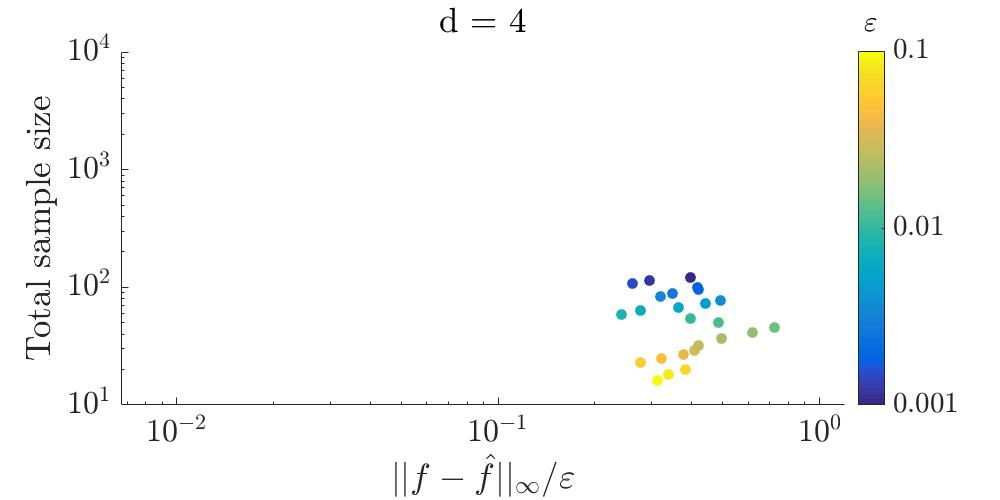
\includegraphics[width=0.7\textwidth]{d4}
\label{fig:four1}
\caption{$f$ is a $d=4$-dim. function with random Fourier coefficients.}
\end{subfigure}
\begin{subfigure}{\textwidth}
\centering
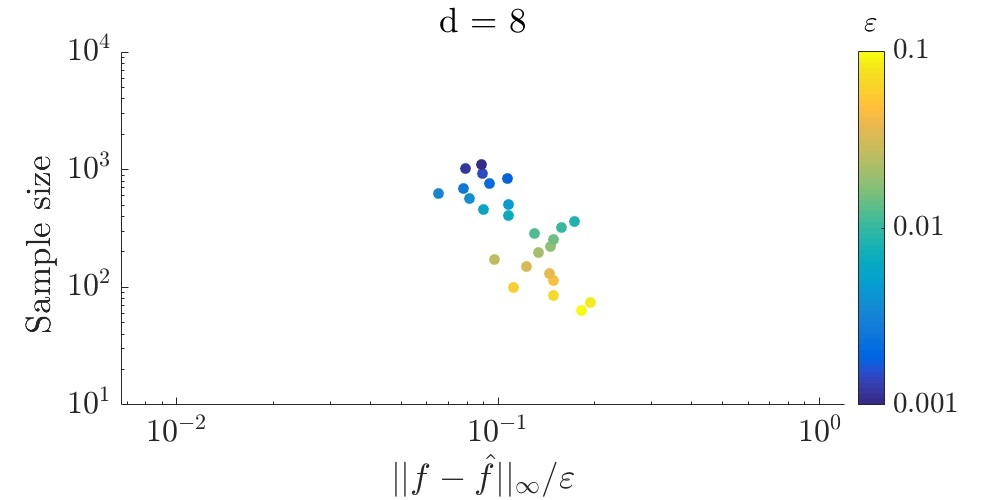
\includegraphics[width=0.7\textwidth]{d8}
\label{fig:four2}
\caption{$f$ is a $d=8$-dim. function with random Fourier coefficients.}
\end{subfigure}
\caption{Adaptive sample size $n^*$ as a function of error ratio $\|f - \hat{f}\|_{\infty}/\epsilon$, with points colored by the absolute error tolerance level $\epsilon$.}
\label{fig:four}
\end{figure}

\begin{acknowledgement}
 P.~Kritzer gratefully acknowledges support by the Austrian Science Fund (FWF) Project  F5506-N26, 
which is part of the Special Research Program ``Quasi-Monte Carlo Methods: Theory and Applications''.
\end{acknowledgement}

\bibliographystyle{spbasic.bst}

\bibliography{ExtraBib.bib,FJH23.bib,FJHown23.bib}

\section*{Appendix}

\end{document}
